%%%%%%%%%%%%%%%%%%%%%%%%%%%%%%%%%%%%%%%%%%%%%%%%%%%%%%%%%%%%%%%%%%%%%
%% This is a (brief) model paper using the achemso class
%% The document class accepts keyval options, which should include
%% the target journal and optionally the manuscript type. 
%%%%%%%%%%%%%%%%%%%%%%%%%%%%%%%%%%%%%%%%%%%%%%%%%%%%%%%%%%%%%%%%%%%%%
\documentclass[journal=jacsat,manuscript=article]{achemso}

%%%%%%%%%%%%%%%%%%%%%%%%%%%%%%%%%%%%%%%%%%%%%%%%%%%%%%%%%%%%%%%%%%%%%
%% Place any additional packages needed here.  Only include packages
%% which are essential, to avoid problems later. Do NOT use any
%% packages which require e-TeX (for example etoolbox): the e-TeX
%% extensions are not currently available on the ACS conversion
%% servers.
%%%%%%%%%%%%%%%%%%%%%%%%%%%%%%%%%%%%%%%%%%%%%%%%%%%%%%%%%%%%%%%%%%%%%
\usepackage[version=3]{mhchem} % Formula subscripts using \ce{}
\usepackage{comment,amsmath,color}
\usepackage{soul}
\usepackage{xcolor}
\usepackage{amssymb}
%%%%%%%%%%%%%%%%%%%%%%%%%%%%%%%%%%%%%%%%%%%%%%%%%%%%%%%%%%%%%%%%%%%%%
%% If issues arise when submitting your manuscript, you may want to
%% un-comment the next line.  This provides information on the
%% version of every file you have used.
%%%%%%%%%%%%%%%%%%%%%%%%%%%%%%%%%%%%%%%%%%%%%%%%%%%%%%%%%%%%%%%%%%%%%
%%\listfiles

%%%%%%%%%%%%%%%%%%%%%%%%%%%%%%%%%%%%%%%%%%%%%%%%%%%%%%%%%%%%%%%%%%%%%
%% Place any additional macros here.  Please use \newcommand* where
%% possible, and avoid layout-changing macros (which are not used
%% when typesetting).
%%%%%%%%%%%%%%%%%%%%%%%%%%%%%%%%%%%%%%%%%%%%%%%%%%%%%%%%%%%%%%%%%%%%%
\newcommand*\mycommand[1]{\texttt{\emph{#1}}}

%%%%%%%%%%%%%%%%%%%%%%%%%%%%%%%%%%%%%%%%%%%%%%%%%%%%%%%%%%%%%%%%%%%%%
%% Meta-data block
%% ---------------
%% Each author should be given as a separate \author command.
%%
%% Corresponding authors should have an e-mail given after the author
%% name as an \email command. Phone and fax numbers can be given
%% using \phone and \fax, respectively; this information is optional.
%%%
%% The affiliation of authors is given after the authors; each
%% \affiliation command applies to all preceding authors not already
%% assigned an affiliation.
%%
%% The affiliation takes an option argument for the short name.  This
%% will typically be something like "University of Somewhere".
%%
%% The \altaffiliation macro should be used for new address, etc.
%% On the other hand, \alsoaffiliation is used on a per author basis
%% when authors are associated with multiple institutions.
%%%%%%%%%%%%%%%%%%%%%%%%%%%%%%%%%%%%%%%%%%%%%%%%%%%%%%%%%%%%%%%%%%%%%
\author{Carlo Andrea De Filippo}
\affiliation{Science Department, University of Roma Tre, Via della Vasca Navale 84, 00146, Rome, Italy}
\email{carloandrea.defilippo@uniroma3.it}

\author{Pietro Corsi}
\affiliation{Science Department, University of Roma Tre, Via della Vasca Navale 84, 00146, Rome, Italy}


\author{Sara Del Galdo}
\affiliation{Science Department, University of Roma Tre, Via della Vasca Navale 84, 00146, Rome, Italy}

\author{Cristiano De Michele}
\affiliation{Physics Department, University of Rome ``La Sapienza'', Piazzale Aldo Moro 2, Rome, Italy}
%\email{cristiano.demichele@roma1.infn.it}

\author{Barbara Capone}
\affiliation{Science Department, University of Roma Tre, Via della Vasca Navale 84, 00146, Rome, Italy}
\email{barbara.capone@uniroma3.it}

%%%%%%%%%%%%%%%%%%%%%%%%%%%%%%%%%%%%%%%%%%%%%%%%%%%%%%%%%%%%%%%%%%%%%
%% The document title should be given as usual. Some journals require
%% a running title from the author: this should be supplied as an
%% optional argument to \title.
%%%%%%%%%%%%%%%%%%%%%%%%%%%%%%%%%%%%%%%%%%%%%%%%%%%%%%%%%%%%%%%%%%%%%
\title[An \textsf{achemso} demo]
  {On the role of Polydispersity on the Phase Diagram of low Density Colloidal Solutions}

%%%%%%%%%%%%%%%%%%%%%%%%%%%%%%%%%%%%%%%%%%%%%%%%%%%%%%%%%%%%%%%%%%%%%
%% Some journals require a list of abbreviations or keywords to be
%% supplied. These should be set up here, and will be printed after
%% the title and author information, if needed.
%%%%%%%%%%%%%%%%%%%%%%%%%%%%%%%%%%%%%%%%%%%%%%%%%%%%%%%%%%%%%%%%%%%%%
\abbreviations{IR,NMR,UV}
\keywords{American Chemical Society, \LaTeX}

%%%%%%%%%%%%%%%%%%%%%%%%%%%%%%%%%%%%%%%%%%%%%%%%%%%%%%%%%%%%%%%%%%%%%
%% The manuscript does not need to include \maketitle, which is
%% executed automatically.
%%%%%%%%%%%%%%%%%%%%%%%%%%%%%%%%%%%%%%%%%%%%%%%%%%%%%%%%%%%%%%%%%%%%%
\begin{document}

%%%%%%%%%%%%%%%%%%%%%%%%%%%%%%%%%%%%%%%%%%%%%%%%%%%%%%%%%%%%%%%%%%%%%
%% The "tocentry" environment can be used to create an entry for the
%% graphical table of contents. It is given here as some journals
%% require that it is printed as part of the abstract page. It will
%% be automatically moved as appropriate.
%%%%%%%%%%%%%%%%%%%%%%%%%%%%%%%%%%%%%%%%%%%%%%%%%%%%%%%%%%%%%%%%%%%%%


%%%%%%%%%%%%%%%%%%%%%%%%%%%%%%%%%%%%%%%%%%%%%%%%%%%%%%%%%%%%%%%%%%%%%
%% The abstract environment will automatically gobble the contents
%% if an abstract is not used by the target journal.
%%%%%%%%%%%%%%%%%%%%%%%%%%%%%%%%%%%%%%%%%%%%%%%%%%%%%%%%%%%%%%%%%%%%%
\begin{abstract}
 The  low-density  phase  diagram  of  nanometric  colloidal  particles  has  a  widespread  range  of applications,  spanning  from  material  science  up  to  biomedical  systems.  Colloids  of  various  shapes have been developed over the last decades either for creating novel devices with peculiar and tunable properties,  such  as  liquid  crystals,  self-assembling  materials  with  particular  optical  properties,  as well as for realising innovative drug delivery carriers [1]. When synthesised, such nanoparticles are always characterised by a non-negligible polydispersity, that might have a non-trivial effect on the properties and clustering of the complex fluids made by such nanomaterials in solution. In  this  work  we  will  address  the  role  played  by  polydispersity  on  the  low volume  fraction equation of state of hard colloidal nanoparticles of various elongations(aspect ratio $A = L/D = [1,5]$) to predict the compressibility of a solution of a drug delivery vessel candidate, namely Au CTAB coated nanorods [2].By means of Monte Carlo NPT simulations we demonstrate that polydispersity on diameter or length of elongated nanoparticles play a diverse role on equation of state (EOS): while a  polydispersity  in  elongation leads to an EOS  comparable  with  the  monodisperse  case, a polydispersity in diameter renders the system overall more compressible with a dependency on the distribution  of  the  diameters. This result is quite  general for anisotropic systems. Moreover,  simulation data have  then  been  strengthened  by a  theoretical  approach based  on  a Parson-Lee approximation of the Onsager theory, that demonstrated to predict quantitatively how the EOS changes with polydispersity with respect to the monodisperse case. Such a result implies that the EOS of a system with a known polydispersity can be quantitively predicted through a  simple  theory starting  from the  EOS  of  the corresponding monodisperse case,  thus  becoming  a powerful tool for both computational and experimental purposes.
\end{abstract}

%%%%%%%%%%%%%%%%%%%%%%%%%%%%%%%%%%%%%%%%%%%%%%%%%%%%%%%%%%%%%%%%%%%%%
%% Start the main part of the manuscript here.
%%%%%%%%%%%%%%%%%%%%%%%%%%%%%%%%%%%%%%%%%%%%%%%%%%%%%%%%%%%%%%%%%%%%%
\section{Introduction}

%Hard functionalised nanoparticles have gathered a great deal of attention over the last decades, due to their widespread applications, spanning from material science up to biotechnology. 
%Nanoparticles have been used, for example,  as drug delivery systems, or they can be designed so to have peculiar optical properties that can be exploited for the realisation of monitoring devices, or they can be foreseen as model system for understanding the properties  viruses (such as the tobacco mosaic).


Design and synthesis of colloidal particles of various sizes, shapes, morphologies and functionalisations is a field that has flourished unprecedentedly over the last decades~\cite{Hueckel2021, Sacanna2013, Manoharan2015, Glotzer2007}. 

% Nanoparticles have seen  important applications in the field of drug delivery [CITA], where functionalised particles can be designed  to release a cargo upon external stimuli, or to attach to specific regions of the cells. Spanning to a completely different field, nanoparticles can be exploited due to their plasmonic resonance [CITA], that has important applications in optoelectronical devices [CITA], or they can be used as a model system  for a variety of complex biological assemblies such as viruses, bacteria or DNA composites [CITA]. 

%FRASE SULLA SHAPE e SU FASI LC
A particularly interesting class of colloids is constituted by nanoparticles of anisotropic shape, whose 
phase diagram is enriched by mesophases such as nematic, smectic, uniaxial columnar phases among many other ones.
These mesophases emerge in different living systems and have been widely exploited in materials science and 
biotechnology.  Prominent examples of anistropic colloids are provided by fd-viruses~(Z. Dogic and S. Fraden,
Langmuir, 2000, 16, 7820–7824), DNA duplexes~(Mine with Stiakakis 2021), cellulose nanocrystals (P. X. Wang, W. Y.
Hamad and M. J. MacLachlan, Nat. Commun., 2016, 7, 11515), polypeptides (XXX), amyloid fibrils (G. Nystrom, M. Arcari
 and R. Mezzenga, Nat. Nanotechnol., 2018, 13, 330–336), collagen (R. Martin, J. Farjanel, D. Eichenberger, A.
Colige, E. Kessler, D. J. S. Hulmes and M. M. Giraud-Guille, J. Mol. Biol., 2000, 301, 11–17) and gold nanorods 
(AuNRs). The latter have proven to be extremely successful when 
medical applications are foreseen, due to their high  biocompatibility and simple 
and versatile synthesis. 

All aforementioned natural or synthetic particles, are characterised by a typical polydispersity that can arise on one or all of the characteristic axes of the colloids. When,  for example, AuNRs are synthesised,  the nucleation process leading to the assembly of the colloidal nanoparticles can give rise to a polydispersity both in the diameter as well as in the elongation of the nanoparticle (\textcolor{red}{AMILOIDI E CELLULOSA}). 

Inspired by such an observation, we focus this work on developing a simple strategy that can be exploited to assess the effect of polydispersity on the phase behaviour of  elongated mesogenic nanoparticles. We thus concentrate on a simple prototypical system constituted of polydisperse hard spherocylinders (HSCs), defined  by means of their elongation  $L$ and their diameter $D$. Every $(L,D)$ combination uniquely defines an aspect ratio $A=L/D$. 

Over the years, the equilibrium properties of HSCs  have been  investigated  experimentally, theoretically 
and numerically; Bolhuis, Frenkel~\cite{Bolhuis1997} and by McGrother~\cite{McGrother96} investigated equilibrium properties of monodisperse hard spherocylinders of length $L$ and diameter $D$; their work  shown that if elongation $A=L/D \gtrsim 3.7$ four stable phases can be found upon increasing concentration: Isotropic (I), Nematic (N), 
Smectic (Sm), and Uniaxial Columnar Crystal (K). Differently, if elongation is smaller than $3.7$,  the Nematic and Smectic phases 
are missing. 
It was then shown that polydispersity can induce profound differences in the phase diagram of HSCs. For example, 
it is known that  length polydispersity in a system of HSCs can inhibit the formation of 
the Smectic phase~\cite{Bates1998}, or, in the case of rod-like particles it can induce a broadening of the IN coexistence region and fractionation~\cite{Lekkerkerker1984,Speranza2002,Wensink2003}. 
Theoretical and numerical predictions on the effects of a $L$ polydispersity on the equations of state,  have been confirmed by experiments on clay rods~\cite{Woolston2015}, bohemite syntethic rods~\cite{Buining1993} and tobacco mosaic virus~\cite{Fraden1993}. 

While great attention has been put in understanding the role of a $L$ polydispersity on the equilibrium properties of HSC, so far the  role played by  a diameter polydispersity has been neglected. We thus focus this work on assessing the role of a $D$ polydispersity on a ($L,D$) polydisperse solution of HSCs on the EOS.
Through a generalised Onsager theory, built on the works of Speranza and Sollich~\cite{Speranza2002}
and of Wensink and Vroege~\cite{Wensink2003}, designed to account for polydispersity , and by means of Monte Carlo (MC) simulations of HSCs, we propose a simple approach to account for polydispersity. 
Benchmarking the phase diagrams with  respect to the monodisperse case, we thus calculate it both theoretically and numerically for a series of polydisperse cases, with particular attention on the  isotropic-nematic transition.
The quantitative comparison between the here presented numerical and theoretical results corroborate the effectiveness of the newly derived simple theory.
Moreover, by analysing separately and contemporary  polydispersities in $L$ and $D$, we surprisingly find that phase behavior is mostly affected by diameter polydispersity of particles rather than length polydispersity. 
% TODO aggiungere qualcosa qui


\subsection{Theory} \label{sec:Theory}
Let us consider a finite density solution of HSCs  characterised by a distribution $P(D)$ of diameters $D$ and a distribution $P(L)$ of lengths $L$.  To define the average elongation we compute $\overline{A}= \int P(D) P(L) L/D dD dL$.
Following Refs.~\cite{Speranza2002,Wensink2003}, we generalize Onsager theory to account for particles polydispersity by introducing a 
size dependent density distribution $\tilde{\rho}(\Omega,L,D)$ defined so that $\tilde{\rho}(\Omega,L,D)d\Omega dL dD $ gives the density of rods with a given $(\Omega,L,D)$ in an interval $dL, dD$ in a solid angle  $d\Omega$. We define such a density distribution as a generalisation for a $L,D$ polydisperse system of the usual orientation distribution $P(\Omega)$ used for monodisperse systems.
%To understand why polidispersities in $D$ and $L$ play such a different role on the EOS, we  generalise, to the polydisperse case,  
%a standard theoretical tool that estimates the equation of state of the solutions through a mean field approach. 
%Even the theoretical approach shows a strong effect of the compressibility correlated to a polydispersity in $D$, while none of the considered distributions for the polydispersity in $L$ affect the EOS.
%Let us start by writing the Helmholtz free energy $F$ of the system, in an isotropic or nematic phase, as [citazioni]:
The Helmoltz free energy within Onsager approach reads:
\begin{equation}
	F = F^\mathrm{id} + F^\mathrm{excl}
\end{equation}

where the first term is ideal gas contribution and the second one is an excess contribution due to particles hindrance.

% The ideal gas contribution is given by

% \begin{equation}
%         \frac{\beta F^{id}}{V} = \frac{\phi}{\overline{v_0}} \ln \left(\frac{\phi}{\overline{v_0}}\right) - \frac{\phi}{\overline{v_0}}
% \end{equation}

The ideal gas contribution can be written as follows:
\begin{equation}
  \frac{\beta F_{id}}{V} = \int d\Omega dL dD\tilde{\rho}(\Omega,L,D) \left [\ln(\tilde{\rho}(\Omega,L,D) \overline{v_0}) - 1 \right]
\end{equation}
while the excess contribution, by resorting to Parsons-Lee approximation~\cite{Parson} in the Onsager theory, is: 
\begin{equation}
\frac{\beta F_\mathrm{ex}}{V} = \frac{1}{2} \, \eta(\phi) 
 \int d\Omega_1 dL_1 dD_2\Omega_2 dL_2 dD_2 \, v_{excl}(\Omega_1,L_1,D_1,\Omega_2,L_2,D_2) \tilde\rho(\Omega_1,L_1,D_1) 
  \tilde\rho(\Omega_2,L_2,D_2)
\end{equation}
where $\phi$ is the volume fraction, $v_{excl}(\Omega_1,L_1,D_1,\Omega_2,L_2,D_2)$ 
is the excluded volume between two spherocylinders with diameters $D_1$
and $D_2$, lengths $L_1$ and $L_2$ and orientations $\Omega_1$ and $\Omega_2$, and
$\eta(\phi) = \frac{1}{4} \frac{4 - 3\phi}{(1 - \phi)^2}$ is the Parson-lee factor.

We know make some assumptions to simplify the analytical calculation of the free energy.
Differently from Refs.~\cite{Speranza2002,Wensink2003}, we assume that the density distribution
$\tilde\rho(\Omega,L,D)$ can be written as follows:
\begin{equation}
\tilde\rho(\Omega, L, D) = \rho(L,D) f(\alpha(L,D), \Omega)
\end{equation}
where $f(\alpha,\Omega)$ is the orientational distribution function which will be equal to $1/4\pi$ in the isotropic phase and 
to the Onsager function in the nematic phase, i.e.:
\begin{equation}\label{eq:Fons}
   f(\alpha,\Omega) = \frac{\alpha}{4 \pi \sinh \alpha} \cosh(\alpha \cos \theta)
\end{equation}
where $\theta$ is the angle between the particle and the nematic axis and $\alpha$ is a non-negative parameter that quantifies the alignment of the system.
We further assume that $\alpha(L,D)=\alpha$, i.e.~that it does not depend on particle size.

According to the assumptions which we made for $\tilde\rho$, the ideal gas contribution to free energy becomes:
\begin{equation}
  F_\mathrm{id} = \int dL dD\,\rho(L,D) \left[\ln(\rho(L,D)\overline{v_0}) - 1\right ] + \frac{\phi}{\overline{v_0}} \, 
  \int \, d\Omega f(\alpha,\Omega) \ln(4 \pi f(\alpha,\Omega))
\end{equation}
where $\overline{v}_0$ is the average volume of the HSCs, i.e.
\begin{equation}
\overline{v}_0 = \frac{V}{N} \int dL dD \rho(L,D) v_0(L, D)
\end{equation}
with $v_0(L, D) = \frac{\pi D^3}{6} + \frac{\pi D^2 L}{4}$.

If one introduces the average excluded volume $\overline{v}_\mathrm{excl}$ defined as follows:
\begin{equation}\label{eq:vex}
\overline{v}_\mathrm{excl} = \left(\frac{V}{N}\right)^2 \int d\Omega_1 d\Omega_2 dL_1 dL_2 dD_1 dD_2\, \tilde\rho_1\, \tilde\rho_2\; v_\mathrm{excl}(L_1, L_2, D_1, D_2, \Omega_1, \Omega_2) 
 \end{equation}
being $\tilde\rho_1=\rho(L_1,D_1) f(\alpha,\Omega_2)$ and $\tilde\rho_2=\rho(L_2, D_2) f(\alpha,\Omega_2)$,
the excess contribution to free energy becomes: 
% \begin{equation}
  % F_\mathrm{ex} = \int d\Omega_1 dL_1 dD_2\Omega_2 dL_2 dD_2 \, v_{excl}(\Omega_1,L_1,D_1,\Omega_2,L_2,D_2) \tilde\rho(\Omega_1,L_1,D_1) 
  % \tilde\rho(\Omega_2,L_2,D_2)
% \end{equation}
 \begin{equation}\label{eq:Fex}
   \frac{\beta F_{ex}}{V} = \frac{1}{2} \, \eta(\phi) \, \overline{v}_\mathrm{excl} \left(\frac{N}{V}\right)^2.
 \end{equation}

%	\iint v_\mathrm{excl}(\gamma[\Omega_1, \Omega_2]) f(\Omega_1)f(\Omega_2) d\Omega_1 d\Omega_2 

We employ the expression provided by Onsager~\cite{onsager1949effects} for $v_\mathrm{excl}$, i.e.

\begin{multline} \label{eq:vexcl}
	v_\mathrm{excl}(L_1, D_1, L_2, D_2, \Omega_1, \Omega_2) = \frac{4}{3} \pi \left(\frac{D_1 + D_2}{2}\right)^3 + \\ + \pi \left(\frac{D_1 + D_2}{2}\right)^2 (L_1 + L_2) + 2 \left( \frac{D_1 + D_2}{2} \right) L_1 L_2 \sin(\gamma)
\end{multline}
where $\gamma=\gamma(\Omega_1,\Omega_2)$ is the angle between the symmetry axes of the two spherocylinders with orientations $\Omega_1$ and $\Omega_2$.

\subsection{Coexistence}

As derived in the previous section, the  total free energy of the system can be expressed as a function of density, and the anysotropy of HSCs gives rise to a series of phases that can either see a homogeneous distribution of particles in solution, or the definition of one or more preferred directions for the nanoparticles. 

The isotropic phase is characterised by a homogeneous distribution of particles in solution. The orientational distribution function is thus equal to $1/4\pi$, and the polydisperse EOS is:

\begin{equation}
	P^* =  - \beta \, \overline{v_0} \frac{\partial F}{\partial V} \Bigg \rvert _{N, T} = \phi + \frac{1}{4} \tilde{v} \phi^2 \frac{2 - \phi}{(1 - \phi)^3} \label{ParsonLee}
\end{equation}

where $\phi=N/V v_0$ is the packing fraction, and   $\tilde{v} = \frac{\overline{v_\mathrm{excl}}}{\overline{v_0}}$ quantifies the deviation to the ideal gas behaviour.

As soon as a local inhomogeneity takes place, particular orientations will be favoured between nanoparticles; this will lead to free energies dependant on both density and on  the average orientation parameter $\alpha$ introduced in  Eq.~\ref{eq:Fons}.
 
It is thus possible to estimate the boundary for the IN transition estimating the coexistence between the two phases as the region defined by the same chemical potential, the same pressure ($\phi_I = \overline{v_0} \rho_I$ and $\phi_N = \overline{v_0} \rho_N$), where the nematic contributions are estimated for the  $\alpha$ value that  minimises the Helmholtz free energy:

\begin{equation}
\begin{cases}
	\frac{\partial}{\partial \alpha}  F_N(\phi_N, \alpha) &= 0\\
	P_I(\phi_I) &= P_N(\phi_N, \alpha) \\
	\mu_I(\phi_I) &= \mu_N(\phi_N, \alpha)
\end{cases}
\end{equation}


%The resulting phase diagram, restricting this evaluation to aspect ratios that can present a nematic phase in a monodisperse system (citazione magari?), is reported in figure \ref{fig:TH_phasediagram}.

%\begin{figure}[!h]
%	\centering
%	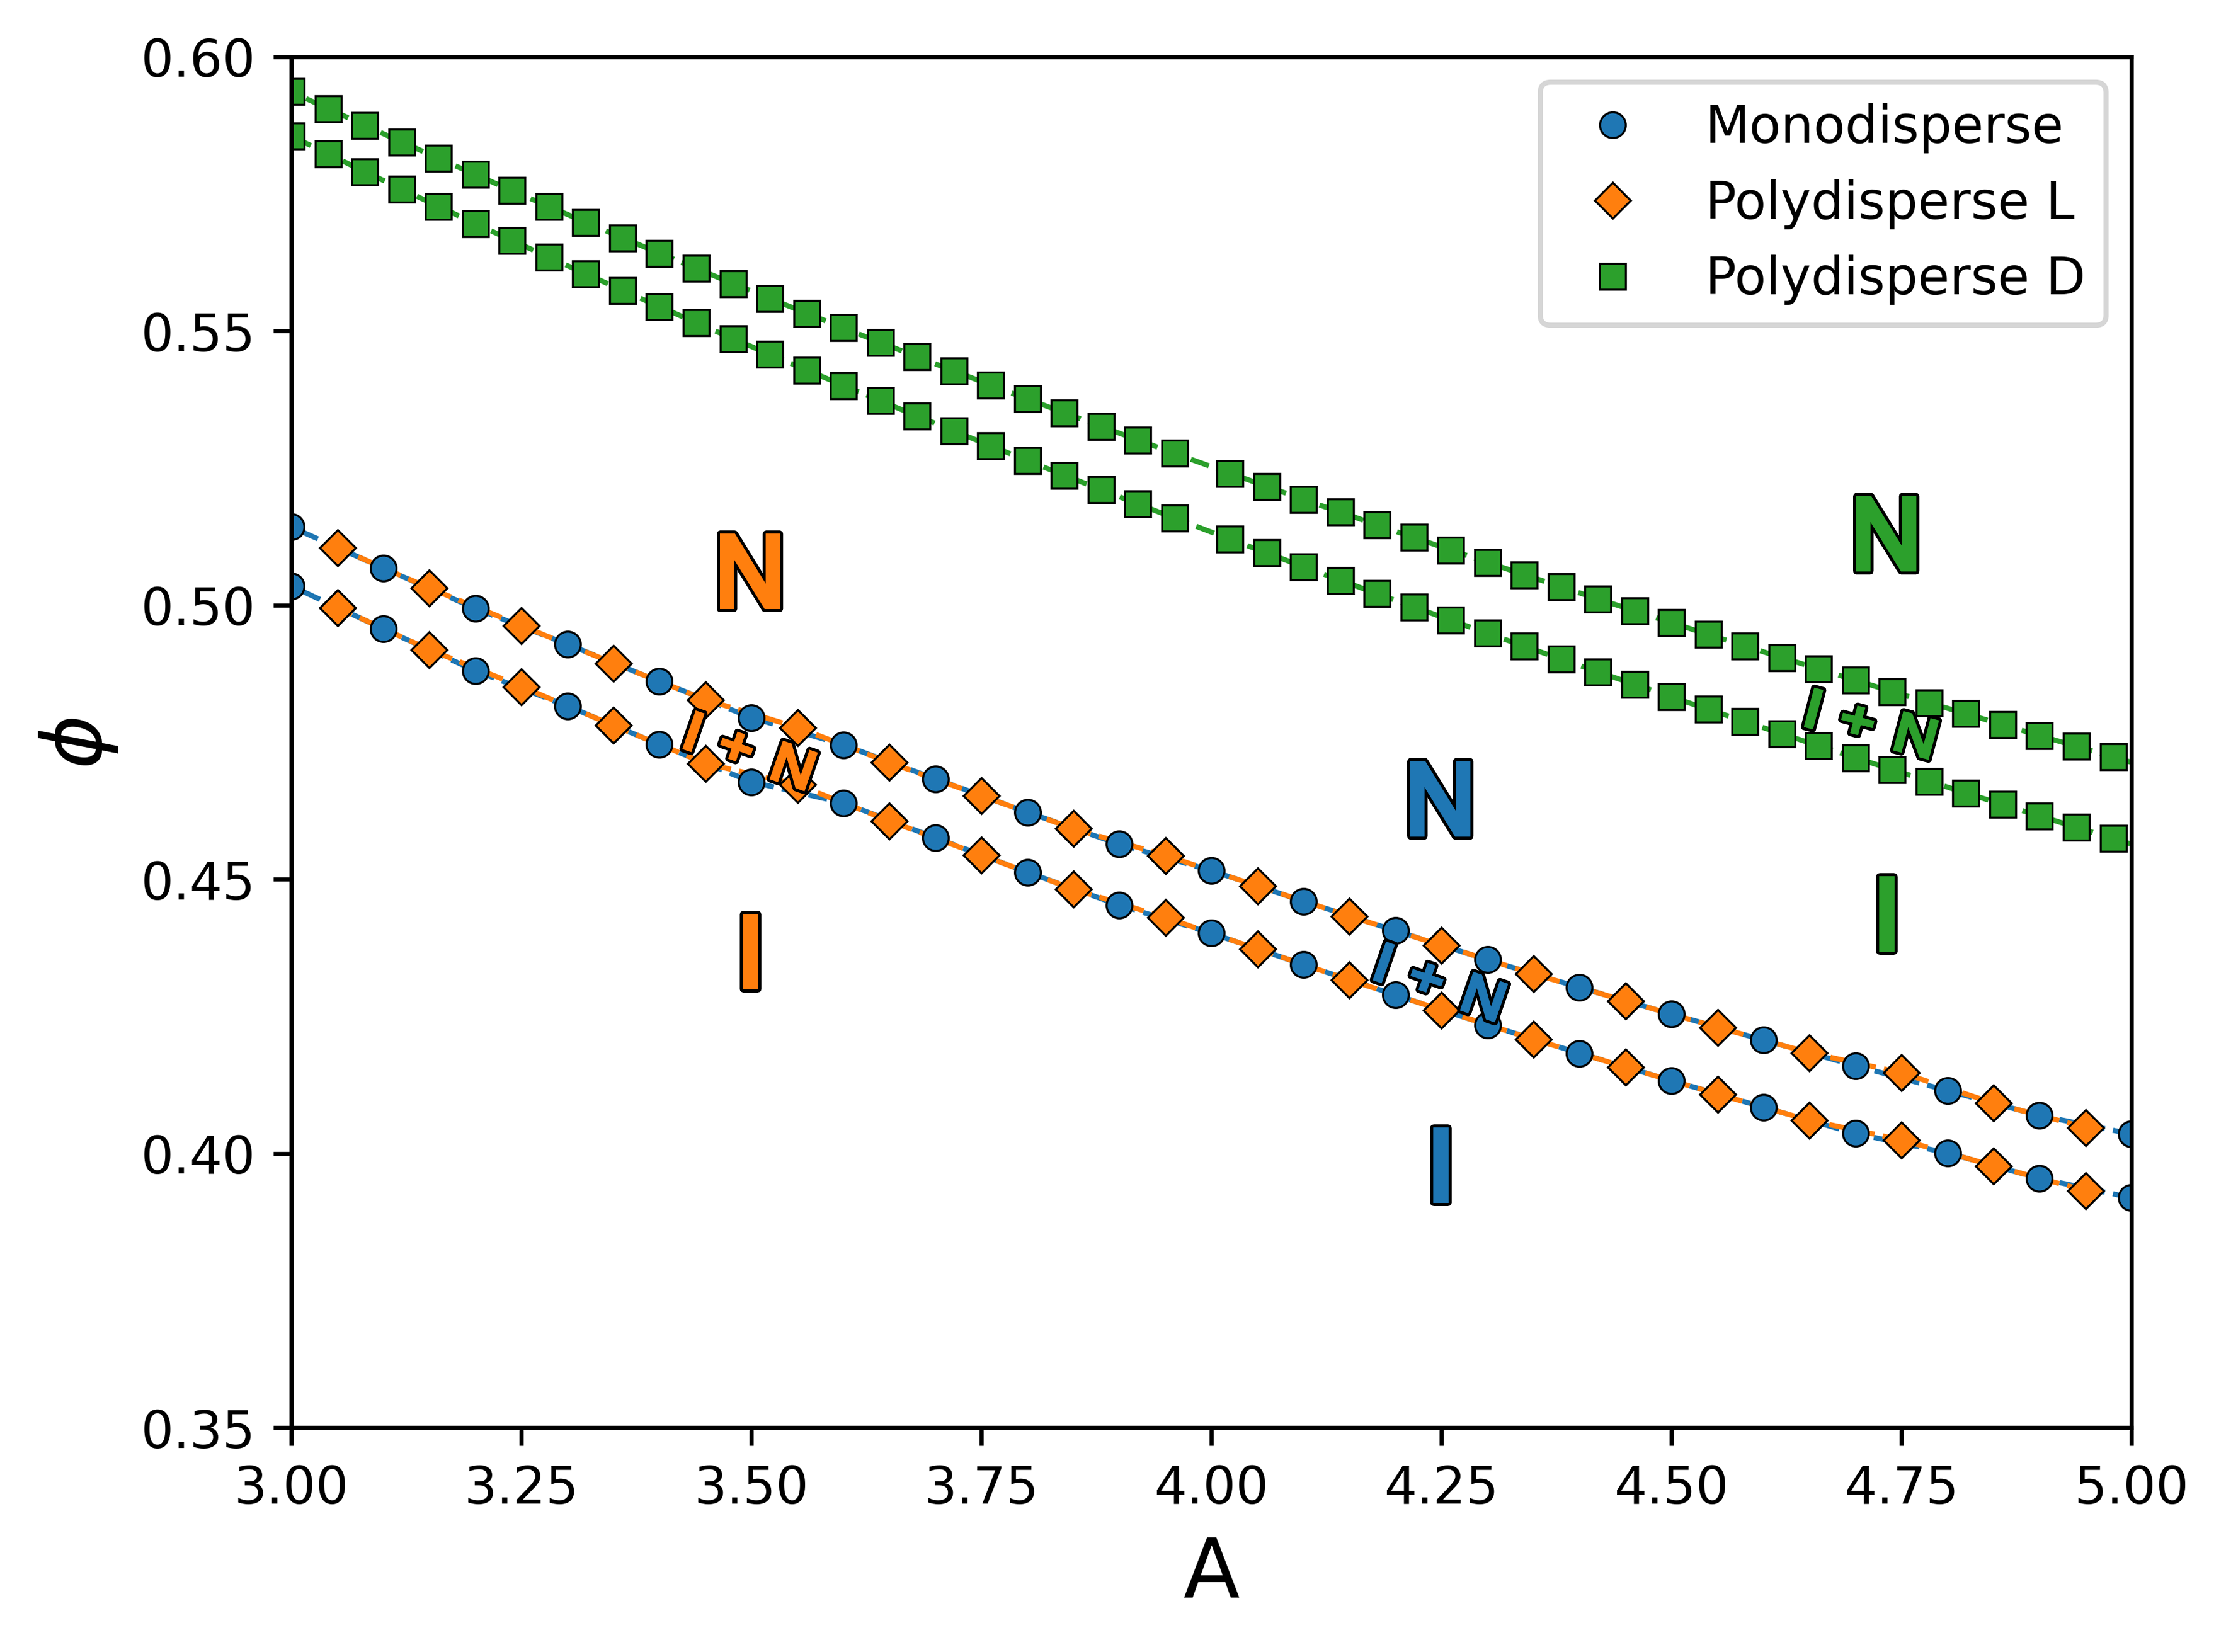
\includegraphics[width=0.9 \columnwidth]{Figures/Phase Diagram3_5.png}
%	\caption{Theoretical phase diagram (around I-N transition) of monodisperse and polydisperse systems.}
%	\label{fig:TH_phasediagram}
%\end{figure}

%Similarly to what we found on the EOS, both by simulations and by a theoretical approach, a polydispersity on $L$ does not affect the I-N coexistence. On the other hand, the introduction of a polydispersity in $D$, which is know to squeeze out the smectic phase \cite{frenkel1998polydispersity}, rises the I-N volume fraction transition, possibly suppressing it (da ampliare).


\subsection{Simulation Technique}
In this paper, we determine the adequacy of the theory outlined in the previous section by appropriate comparisons with  computer simulation data for polydisperse hard spherocylinders. As in the theoretical section, we deeply explore the effect of polydispersity  by comparing the results obtained for the equation of state for monodisperse systems (that we set as a benchmark) to the equilibrium properties obtained for polydisperse hard spherocylinders. In particular we set an in depth analysis focused at unveiling the role played by a polydispersity in diameter and in elongation, by analysing both properties of $L$ (or $D$) polydisperse nanoparticles, as well as hard colloids that are contemporary polydipserse both in $D$ as well as in $L$. 

We thus perform extensive Monte Carlo simulations in the isothermal-isobaric NPT ensemble, where full isotherms are obtained by compression of the systems from the low-density isotropic fluid.


The analysis is motivated by the typical polydispersity arising during the synthesis of experimental NPs: the nucleation process leading to the assembly of the colloidal nanoparticles can give rise to a polydispersity both in the diameter as well as in the elongation of the nanoparticle, as exemplified in  Fig. \ref{fig:HSC_model}, where one amongst all possible polydispersity distributions for the nanoparticles is reported, together with a snapshot of a  polydisperse spherocylindrical solution  in an isotropic phase. 
\begin{figure}[!ht]
    \centering
    %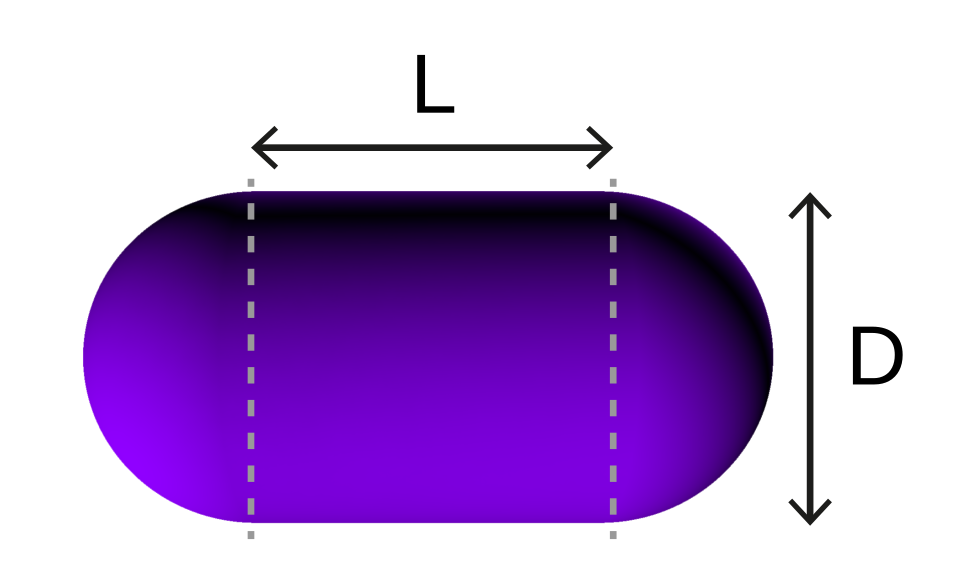
\includegraphics[width=0.25 \columnwidth]{Figures/A1_scheme.png}
    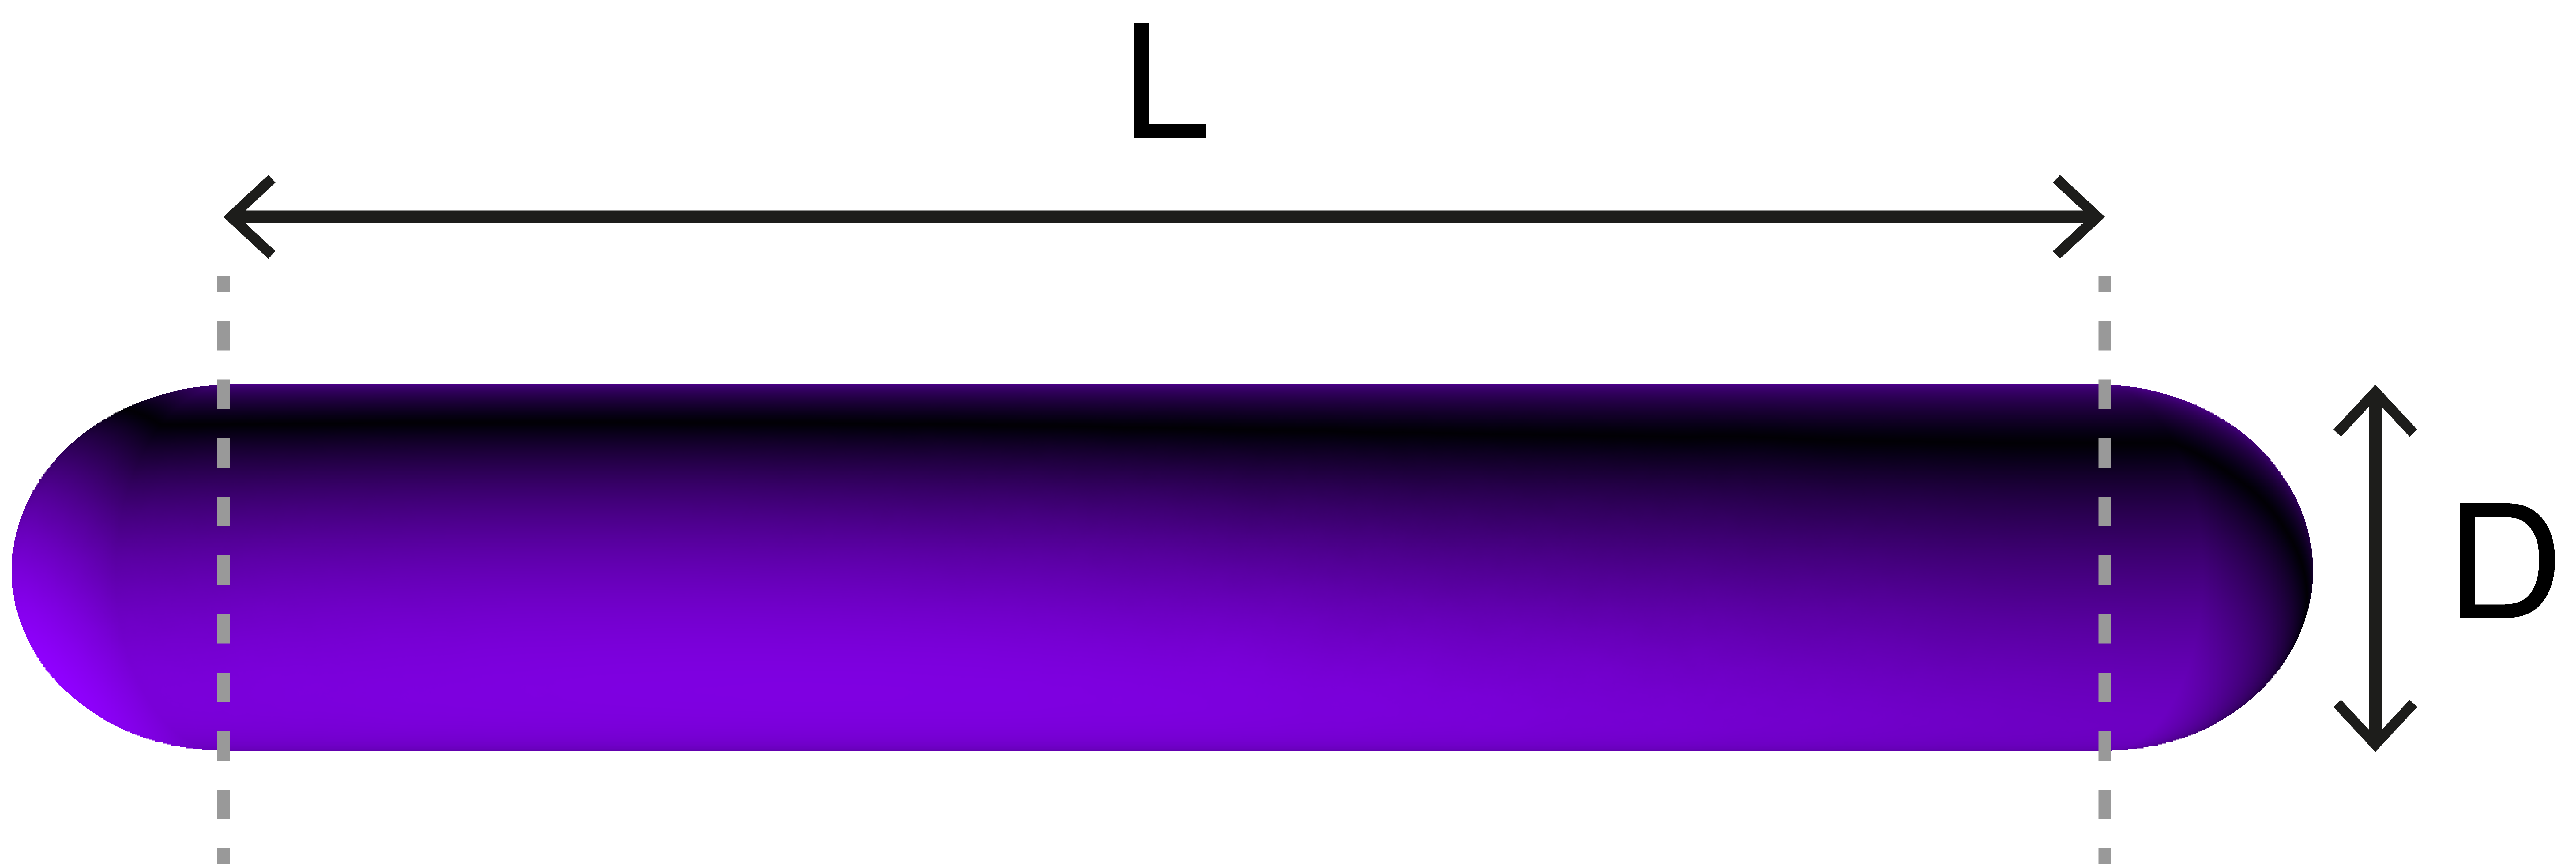
\includegraphics[width=0.2 \columnwidth]{Figures/A5_scheme.png}
    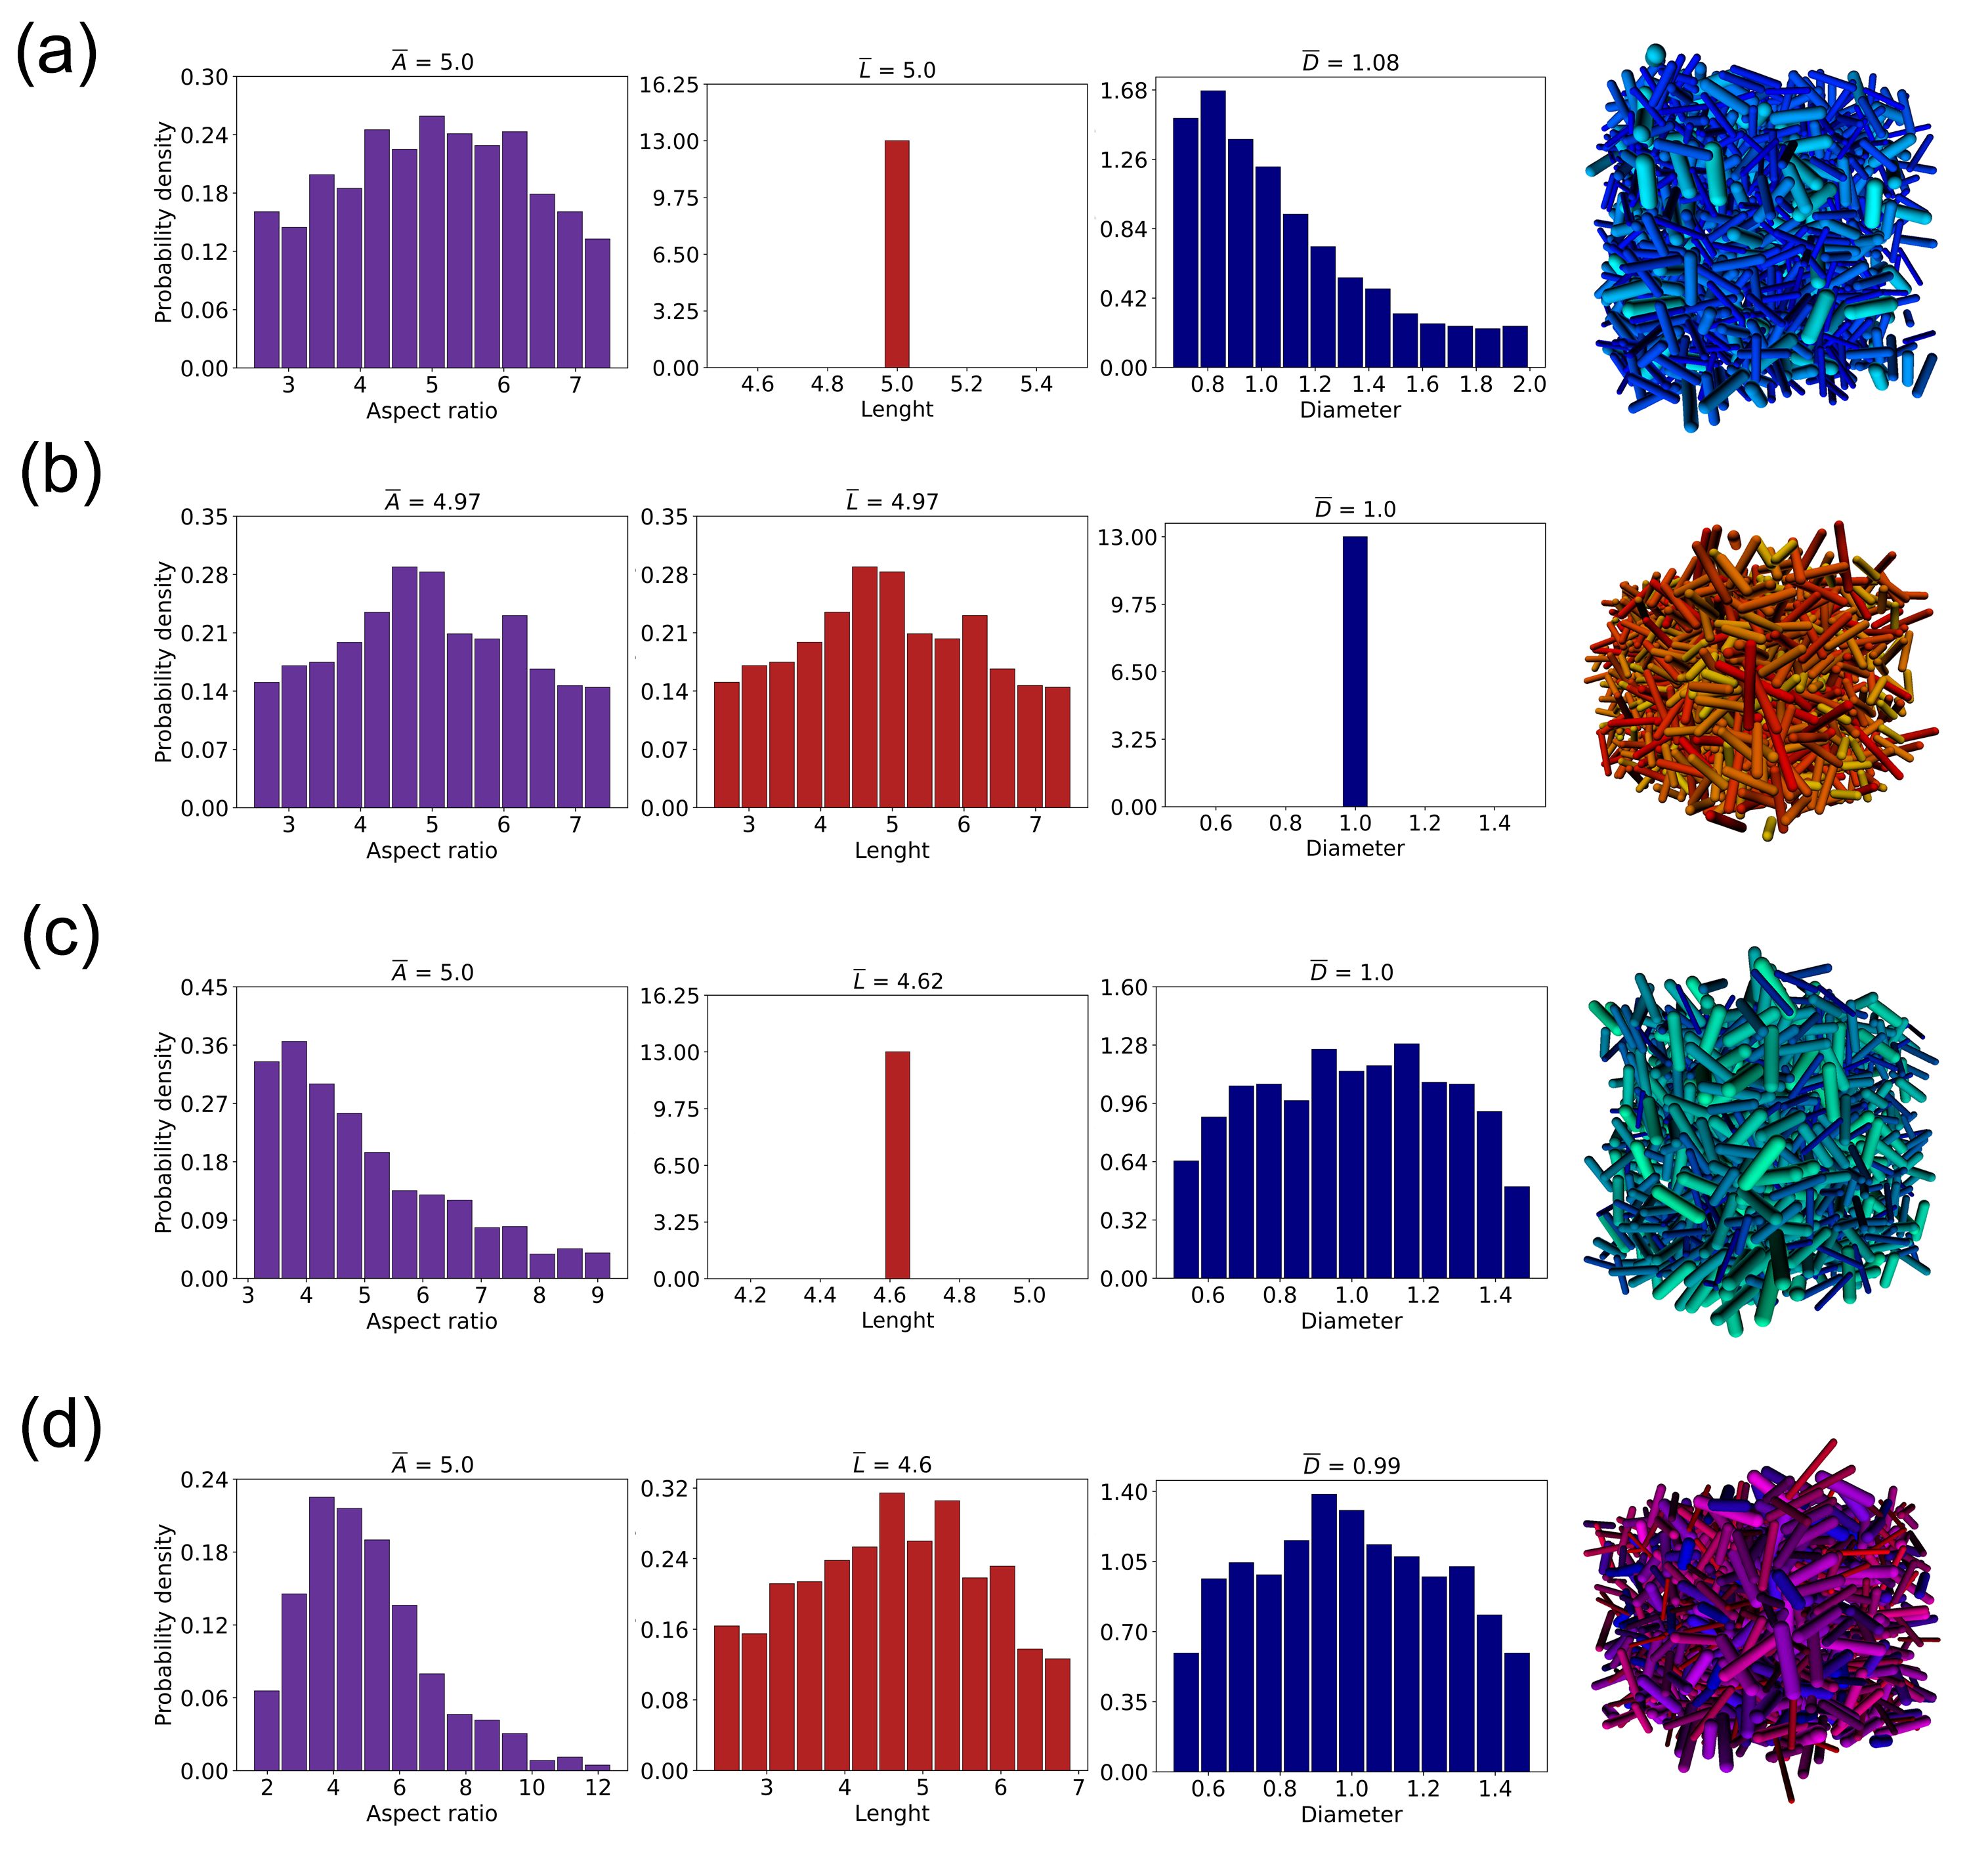
\includegraphics[width=0.7\columnwidth]{Figures/Polydisp_hist.png}
    \caption{We here report for clarity reasons, a particular case of polydispersity  in $A$ (deriving from polydispersities on both $D$ and $L$) and a snapshot of the polydisperse system  in an isotropic phase ($P^*=1$). In particular the reported case is $\bar{A}=5$. We do not report in the main text of the article all the polydispersity types that we analysed, but we describe  them extensively  in the SI.}
    \label{fig:HSC_model}
\end{figure}

We will undergo an in depth analysis on the role played by  polydispersity  on the phase diagram; particles can be polydisperse in  $D$ as well as in $L$. This will induce a polydispersity on the aspect ratio  $A = L/D$. As in the monodisperse case, the aspect ratio is the parameter identifying the nanoparticles that plays the major role when phase transitions occur,  we will in the following classify systems acconding to their average aspect ratio. To set the benchmark for our analyses, we compute the (known) phase diagram for the monodisperse case, starting from extremely low densities  up to concentrated solutions (over the isotropic/nematic transition). We thus perform hybrid NVT-NPT Monte Carlo (MC) simulations to estimate the equilibrium properties of systems described by an aspect ratio $A \in [1, 5]$ for solutions of either $N = 1296$ or $2500$ colloids.  
The inter-particle repulsion, due to the non penetrability of the NPs,  is modelled as an hard core potential that is estimated through the Vega and Lago algorithm \cite{VegaHSC1994}. 
 Systems are equilibrated in the NVT ensemble; then the equilibrated  configuration is moved in an isothermal-isobaric ensemble  (NPT), so that the system is free to attain its equilibrium volume for each simulated pressure $P$. 
 \textcolor{red}{ questo va messo negli SI - 
 Every MC cycle is made by $N$ steps, where $N$ is the total number of particles. One MC step in the NVT ensemble consist of $50\%$ trial random displacement  and $50\%$ random reorientations for each  particle, while in the NPT ensemble the MC moves will consist in  $1/N$ trials in volume change, and all remaining moves will be equally distributed between random displacements and orientations. 
	The volume move consists in an anisotropical change of  one  side of the box chosen randomly. Anisotropic moves are chosen not to introduce any artificial order in the system \cite{frenkel.md.book.1996}. 
	}
Phase diagrams are computed as a function of the  reduced pressure  $P^* = \beta P v_0$, where $\beta = 1/(k_\mathrm{B} T)$, $k_B$ is the Boltzmann constant, and $v_0$ is the volume of a single particle and the packing fraction, $\phi = v_0 \, \rho = v_0 \, N / V$. 
The Equation of State (EOS) is thus  estimated  by computing the equilibrium  packing fractions $\phi$ for every given reduced pressure $P^* $. 

We focus on reduced pressures  $P^* = \beta P v_0 \in [0.01; 15]$ that span from below to above the Isotropic Nematic (I-N) transition, that, if present, is know to be in the region  $5 \geq P^* \leq 10$ for the $A\in[1,5]$ cases \cite{Bolhuis1997, Jackson1996}. 

Once set the benchmark for out work by computing the EOS for the monodisperse case, we extend our analysis to the effect introduced by  polydispersity on the equilibrium properties of the system. 

We thus introduce polydispersity either separately or simultaneously in $D$, in $L$, thus inducing a polydispersity in $A$. A detailed description of all of the considered combinations for the various polydispersities is reported in the SI. 
All polydispersities are chosen so that the average value the aspect ratio $\overline{A}$ can be directly compared to the monodisperse case. 
As polydispersity can affect both the compressibility of the system in the case of dilute solutions, as well as the isotropic nematic transition, we first analyse separately the two cases.

\subsection{The role of polydispersity in  solutions below the isotropic Nematic Transition}
We start by analysing the effect played by a wide set of polydispersities on the EOS of dilute systems ($P^*<5$) for the $A\in [1,5]$ cases. Cases in which polydispersities is present on $L, D$ and consequently in $A$ are analysed together with cases in which either $L$ or $D$ are kept monodisperse still inducing a polydispersity in  $A$. 
As reported in Fig.\ref{fig:EOS_HSC_comparison} for two out of all the analysed cases (all other cases are reported in the SI), it is immediate to notice that polydispersities in $D$ and $L$ play a completely different role. While  even extreme polydispersities in $L$ (up to $75\%$)  do not affect at all the EOS computed for the monodisperse case, even a small polydispersity in $D$ increases dramatically the compressibility of the system.
Comparing the monodisperse EOS with all of the polydisperse $D$ cases, the system shows  a higher equilibrium packing fraction $\phi$ in the case of polydispersity in $D$ for every  pressure $P^*$; moreover, the EOS depends on the particular polydispersity distribution of the diameters. We will address extensively  this point in the theoretical section.

\begin{figure}[!h]
    \centering
    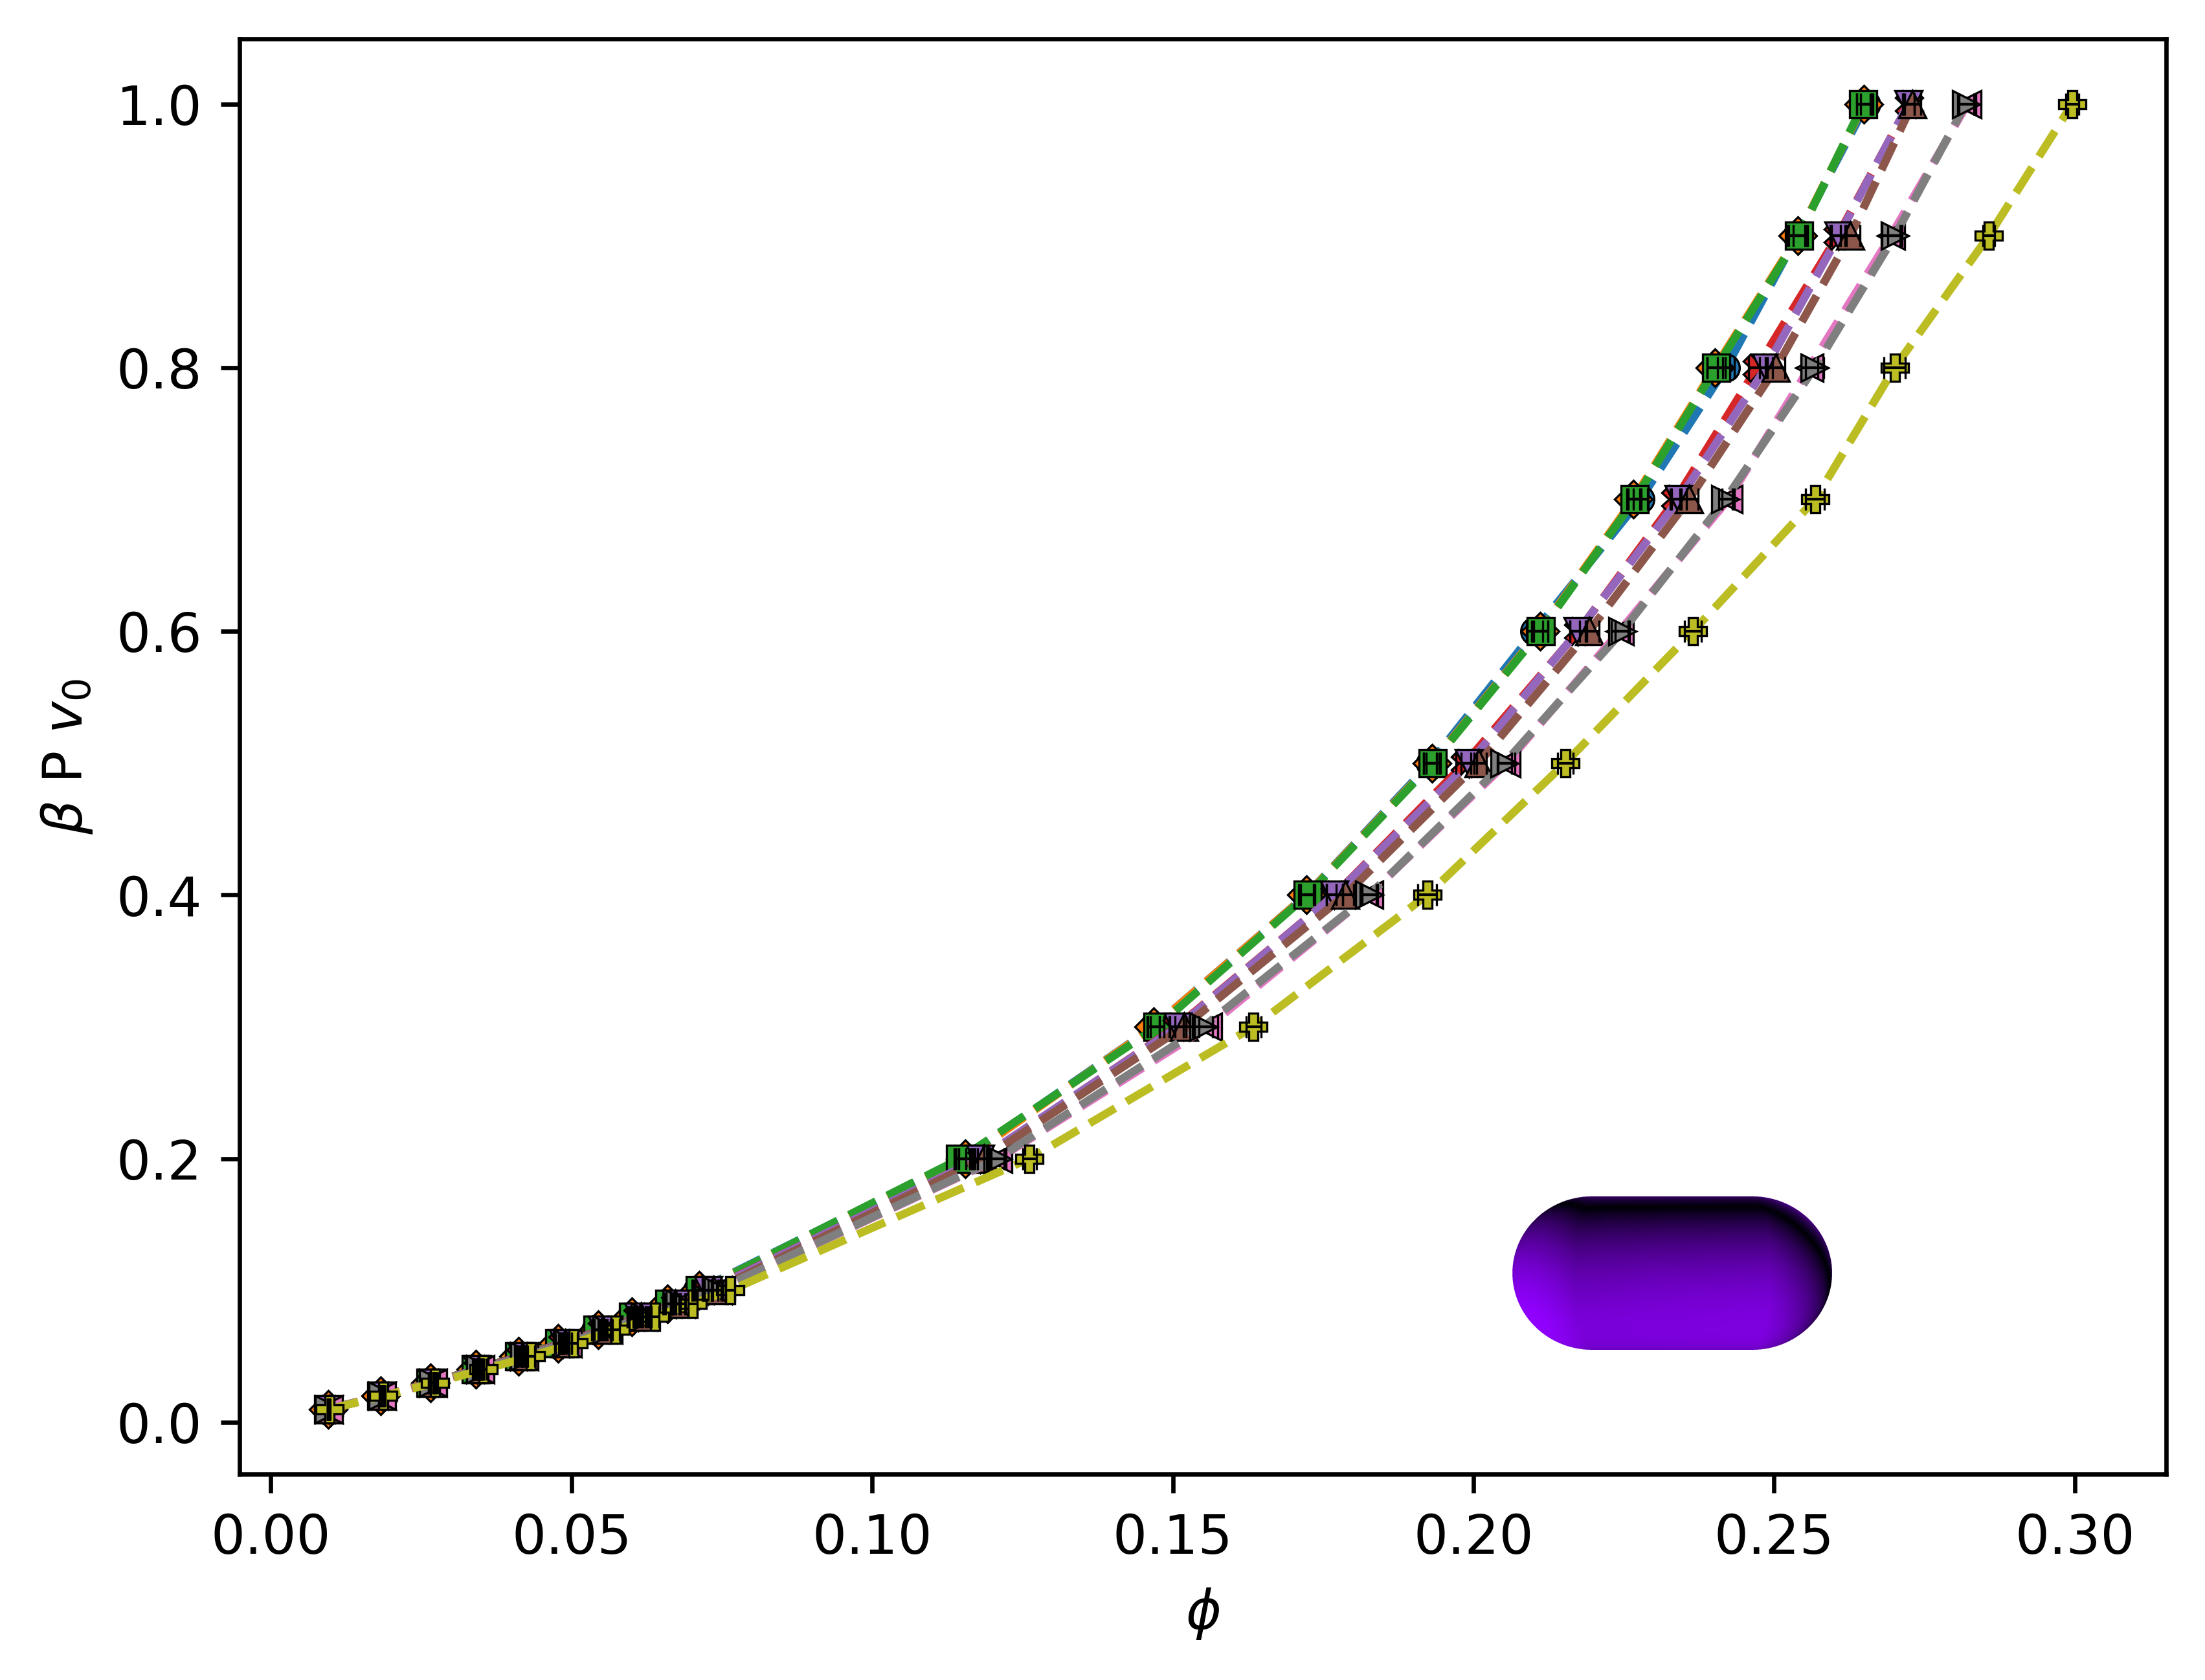
\includegraphics[width=0.45 \columnwidth]{Figures/EOS_A1.png}
    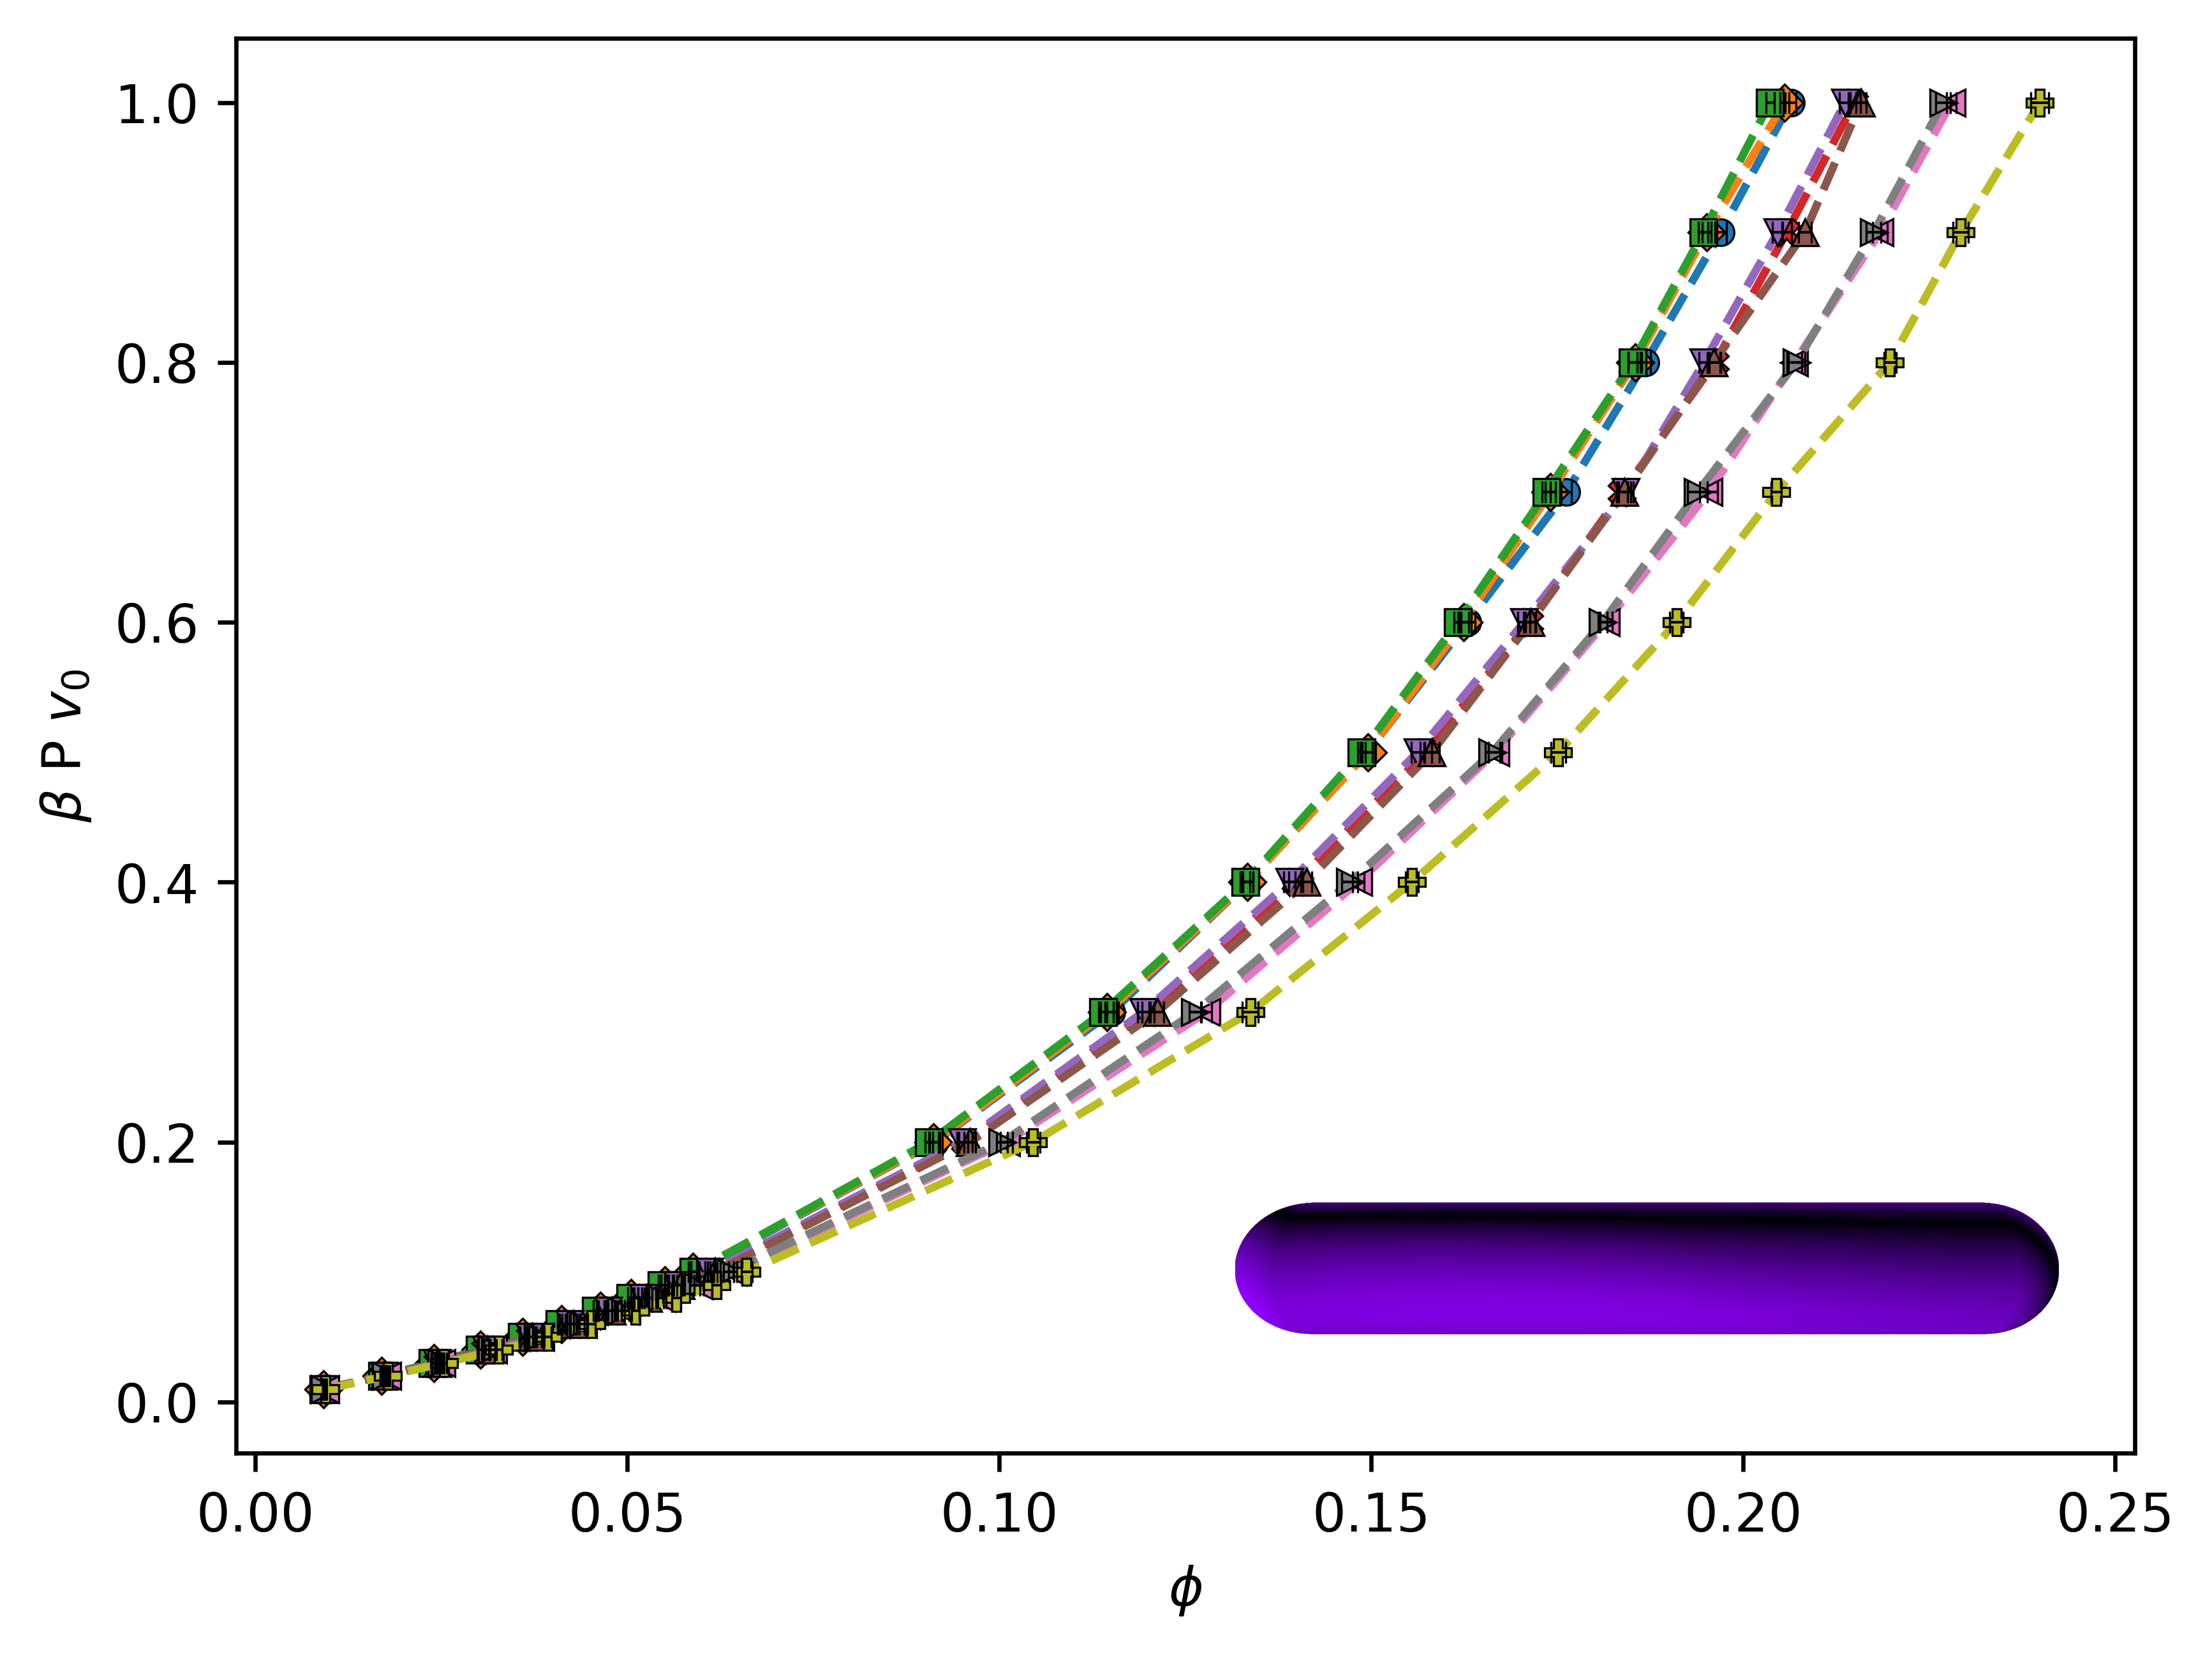
\includegraphics[width=0.45 \columnwidth]{Figures/EOS_A5.png}
    \caption{Equation of state of the systems analysed in this work for $A = 1$ (right) and $A = 5$ (left): monodisperse (circles), polydisperse L (diamonds), polydisperse L 75 \% (squares), Gauss polydisperse D (x symbols), Gauss polydisperse D and L (downward triangles), polydisperse D (upward triangles), Gauss polydisperse D 75 \% (leftward trinagles), Gauss polydisperse D and L 75 \% (rightward triangles), and polydisperse D 75 \% (plus symbols).  (Aggiungere un inset con la magnification in alto a sinistra?)}
    \label{fig:EOS_HSC_comparison}
\end{figure}
We perform local and global analyses to the system to assess whether any local pre-ordering is present for the low packing fractions analysed. We thus computed the nematic order parameter $S$ that is almost zero for all analysed cases and all polydispersities (more details in the SI). Some interesting information on the arising of a pre-nematic transition, can be seen by computing theorientational radial pair distribution function $g_2(r)$, defined as  
\begin{equation}
g_2(r) = \langle P_2 (\cos(\theta_{ij}(r))\rangle
\end{equation}
where $P_2$ is the second order Legendre polynomial $P_2 (\cos(\theta_{ij}(r)) = (\cos^2(\theta_{ij}(r)) - 1)/2$, $\cos(\theta_{ij}(r)) = \boldsymbol{u}_i \cdot \boldsymbol{u}_j$,  and $\theta_{ij}(r)$ is the angle between the main axes  $\boldsymbol{u}_i$ and $\boldsymbol{u}_j$ of the $i$-th and $j$-th particles, and  $r$ is the distance between the  centres of masses of two particles. 
While the nematic order parameter $S$ provides information over the emergence of an eventual ordering of the whole solution,  $g_2(r)$ provides information eventual alignment of the particles one with respect to the other. 

The analysis of $g_2(r)$ shows that, notwithstanding no global nematic order is present in the system, anisotropy introduces the breaking of the global symmetry with a consequent local pre-ordering between particles, even in extremely dilute solutions. While no nematic order is shown by any of the analysed systems in the considered range of the packing fraction,a first analysis of $g_2(r)$ (see SI for details) shows the emergence of a local alignment between the nanoparticles that is enhanced by a higher value of $A$: as soon as $\phi >\phi^*$, local rotational freedom is lost and nanoparticles start aligning one with respect to the other. The local alignment involves a number of particles that is an increasing function of $A$: the more the nanoparticles are anisotropic the higher the number of particles that start aligning locally one with respect to the other.   Particles align along $L$, but in the low packing fraction regime, there is no long range order (see SI for the extensive analyses of the pair distribution functions $g(r)$). For such a reason, it is to be expected that - at low packing fraction - a  polydispersity in $L$ should not  affect extensively the global properties of the solution. 
Differently,  the emergent pre-alignement involves an the average distance between particles that is dominated by $D$. For such a reason not only the polydispersity in $D$ changes the global properties of the solution, but different polydispersities might induce  different local and global effects, as was pre-announced in the EOS. The discussed results are reported  the $A=5$ case in figure\ref{fig:G_or_A5}. It is here possible to appreciate that the emergence of a local alignment is not suppressed by any of the polydispersity analysed, neither in $D$ or in $L$;  while local order is always present,  a polydispersity in the diameter affects the width of the distribution.
  \begin{figure}[!h]
    \centering
    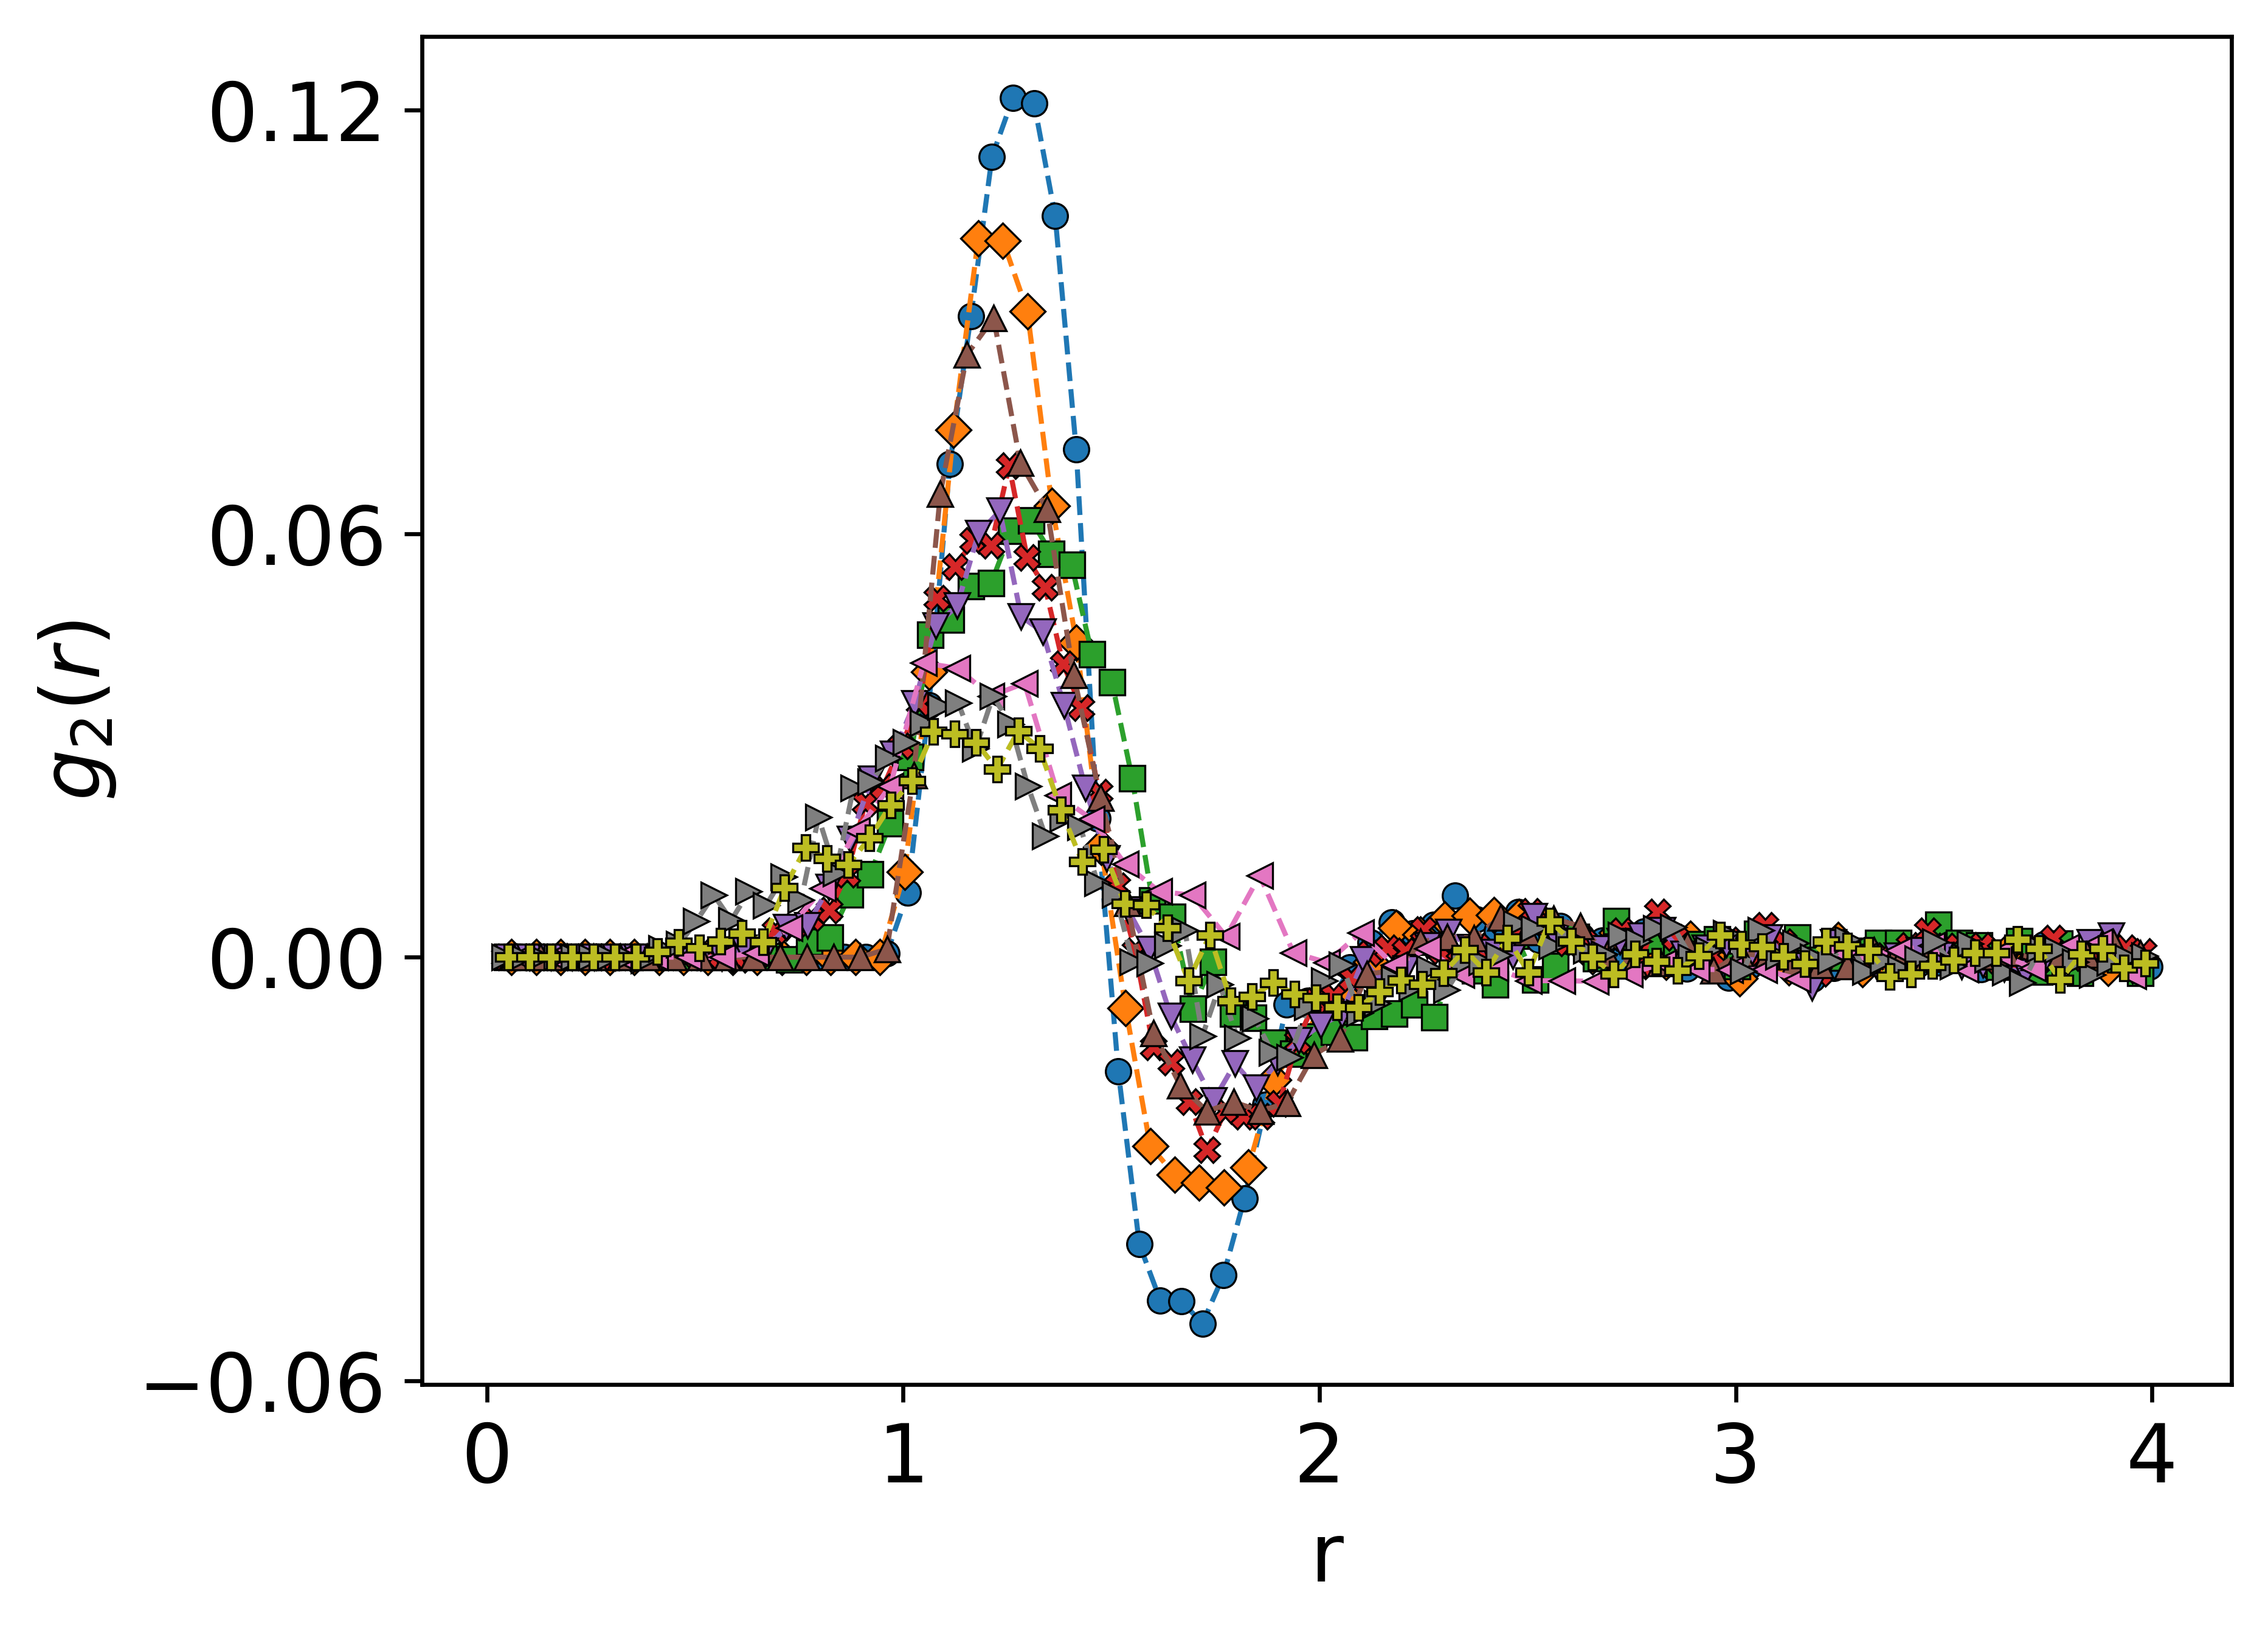
\includegraphics[width=0.45 \columnwidth]{Figures/G_or_A1.png}
    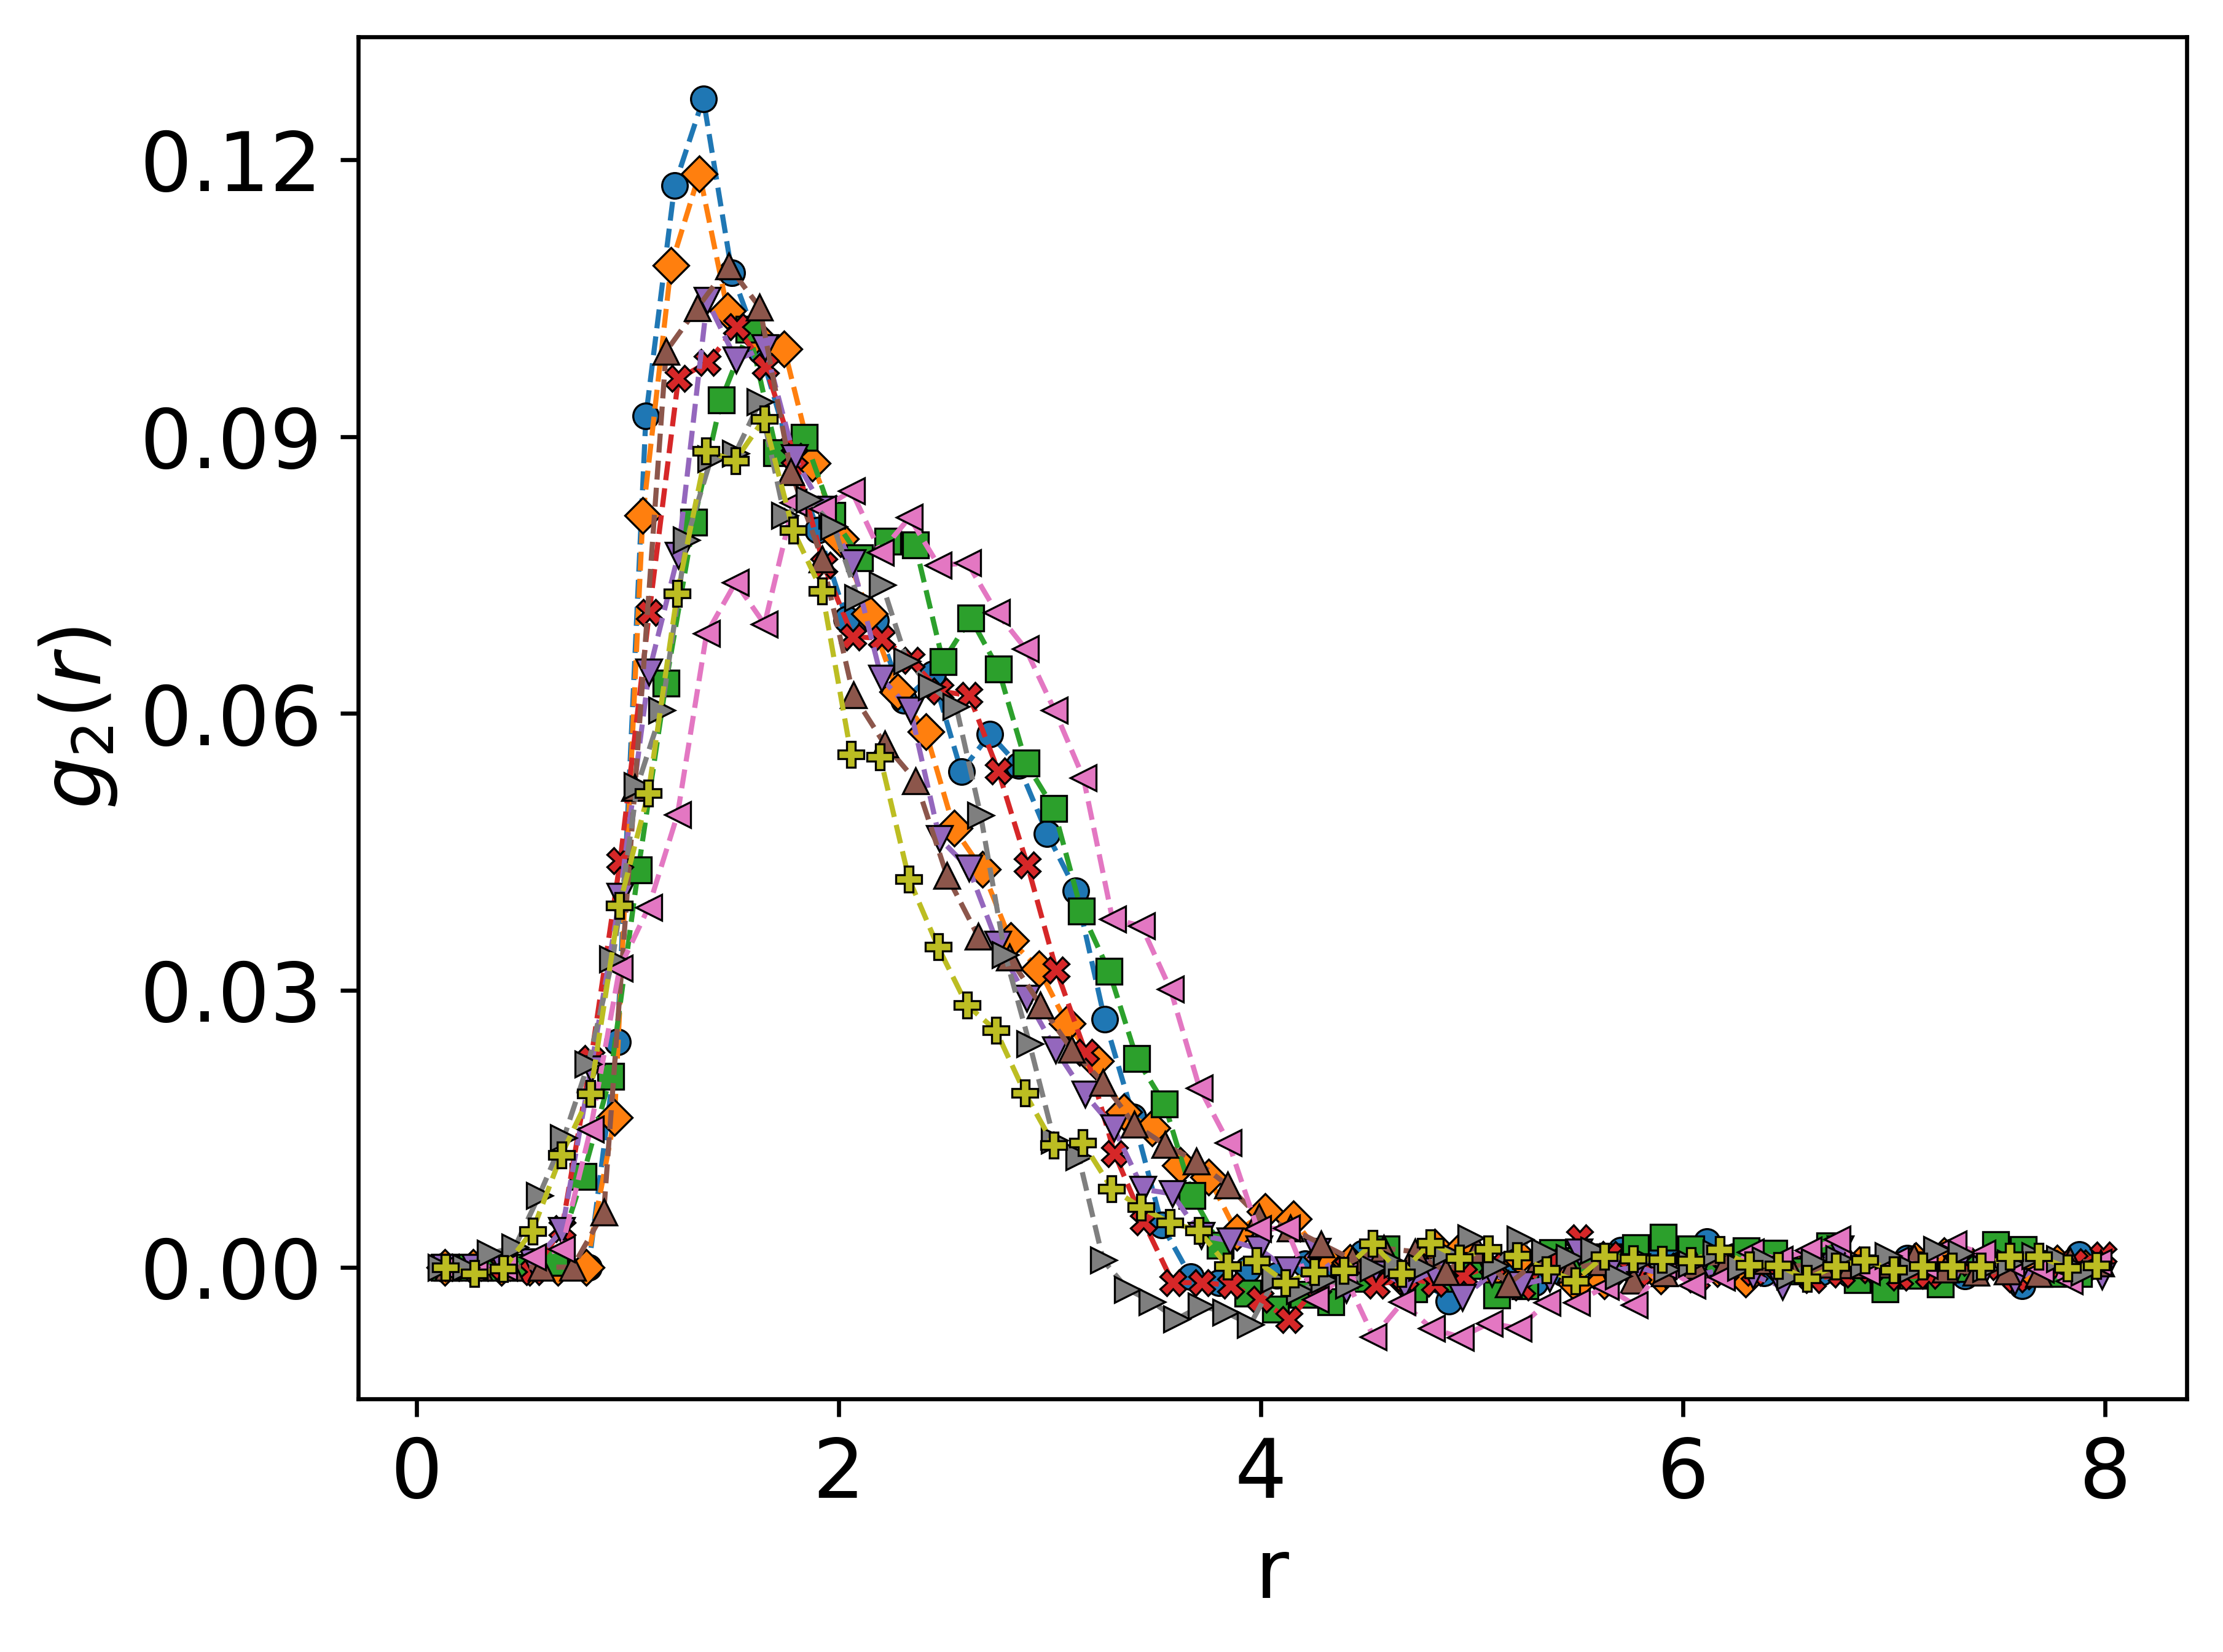
\includegraphics[width=0.45 \columnwidth]{Figures/G_or_A5.png}
    \caption{Orientational pair radial distribution function $g_2(r)$ as a function of the inter-particle distance $r$ for  $\overline{A}=5$  compared to the monodisperse $A=5$ case DIRE CHE SONO I COLORI SE VOGLIAMO METTERLA - IO LA METTEREI.}
    \label{fig:G_or_A5}
\end{figure}
 
The emergence of local alignment between particles  only gives a first glimpse on the reason for which the polydisperse phase diagram for low $\phi$ is almost unaffected by a polydispersity in $L$, while it is dominated by the polydispersity in $D$. As particles align locally but, no global nematic order arises due to the low concentrations, the ``noise'' introduced by polydispersity on $L$ is not felt by the global properties of the solution, while the one on $D$ affects the average distance between the slightly oriented clusters of particles, thus affecting the global compressibility of the system. 
A more in depth explanation of the reason for the diverse role covered by $D$ and $L$ in the EOS is provided in section \ref{sec:Theory}. 

%From the analysis of the pair distribution function between all particles, it is shown that solutions of slightly anisotropic particles behave similarly to solution of spherical colloids, so that a fluid phase emerges, as $A$ increases, the homogemeous liquid like behaviour is lost.  
%The emergence of local alignment between particles is part of the explanation on  why the polydisperse phase diagram for low $\phi$ is almost unaffected by a polydispersity in $L$ and dominated by the polydispersity in $D$: as particles align locally but, no global nematic order arises due to the low concentrations, the ``noise'' introduced by polydispersity on $L$ is not felt by the global properties of the solution, while the one on $D$ affects the average distance between the slightly oriented clusters of particles, thus affecting the global compressibility of the system. 

We report in table \ref{tab:vtilde} the average excluded volume, the mean particle volume, and the ratio $\tilde{v}=\overline{v_\mathrm{excl}}/\overline{v_0}$ for all of the polydispersities analysed in this work (only $\overline{A} = 5$ for clarity). It appears that $\tilde{v}$ is unaffected by any $L$ polydispersity, while all of the different considered polydispersity distributions in $D$ contribute to obtain a different $\tilde{v}$.

\begin{table}
	\begin{tabular} { | c | c | c | c | }
		\hline 
		System type& $\overline{v_\mathrm{excl}}$ & $\overline{v_0}$ & $\tilde{v}$ \\
		\hline
		Monodisperse & 74.875 & 4.451 &  16.824 \\
		\hline
		Polydisperse L & 74.875 & 4.451 & 16.824  \\
		\hline
		Polydisperse L 0.75 & 74.875 & 4.451 & 16.824 \\
		\hline
		Polydisperse D Gauss & 68.334 & 4.517 & 15.128 \\
		\hline
		Polydisperse D L Gauss & 68.334 & 4.517 & 15.128 \\
		\hline
		Polydisperse D & 86.725 & 5.835 & 14.863 \\ 
		\hline
		Polydisperse D Gauss 0.75 & 58.226 & 4.437 & 13.124 \\
		\hline
		Polydisperse D L Gauss 0.75 & 58.226 & 4.437 & 13.124 \\
		\hline
		Polydisperse D 0.75 & 116.000 & 10.008 & 11.591 \\
		\hline
	\end{tabular}
	\caption{\label{tab:vtilde} Comparison of $\overline{v_\mathrm{excl}}$, $\overline{v_0}$ and $\tilde{v}$ computed theoretically via Mathematica in the case of $\overline{A} = 5$ for the simulations presented in this work.}
\end{table}

This behaviour has been found for all the aspect ratios analysed, as reported in figure \ref{fig:vtilde}.

\begin{figure}[!h]
	\centering
	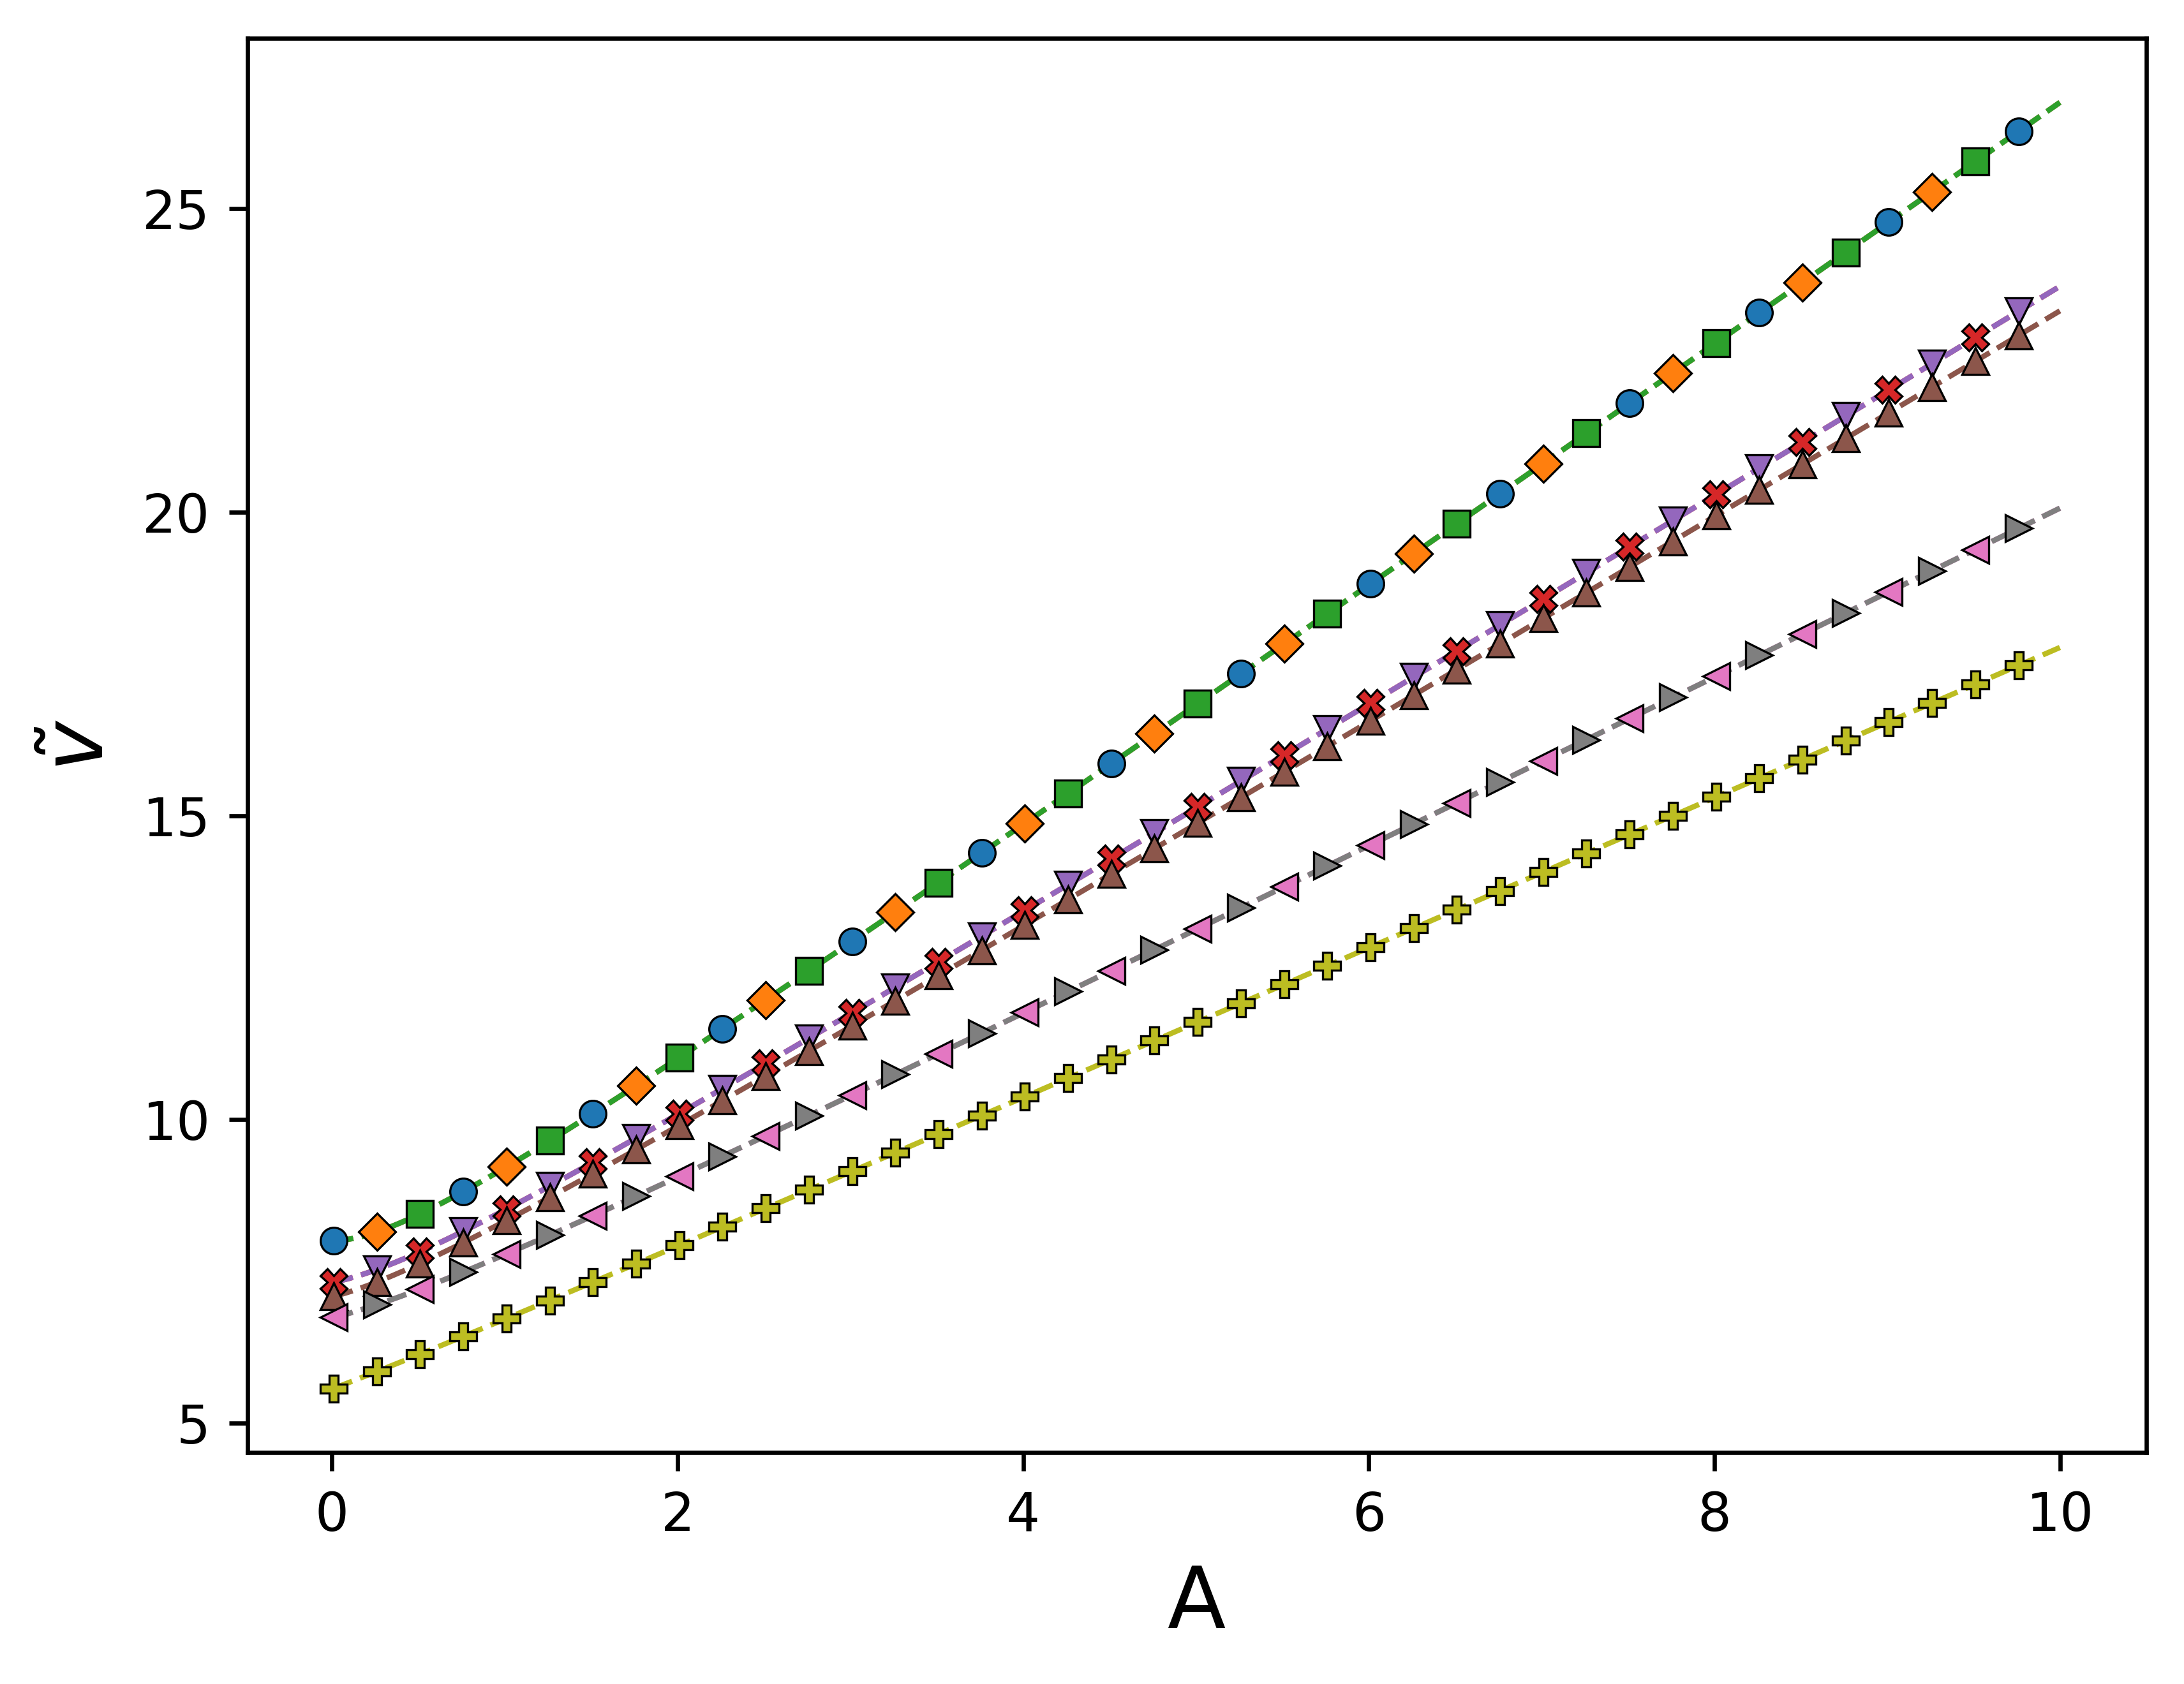
\includegraphics[width=0.9 \columnwidth]{Figures/vtilde.png}
	\caption{Values of $\tilde{v}$ as a function of $\overline{A}$ for the system studied in this work.}
	\label{fig:vtilde}
\end{figure}

These pattern is mirrored in the theoretical isotropic EOS of our systems which are qualitatively in agreement with our MC simulations, as seen in figure \ref{fig:TH_EOS}.

\begin{figure}[!h]
	\centering
´	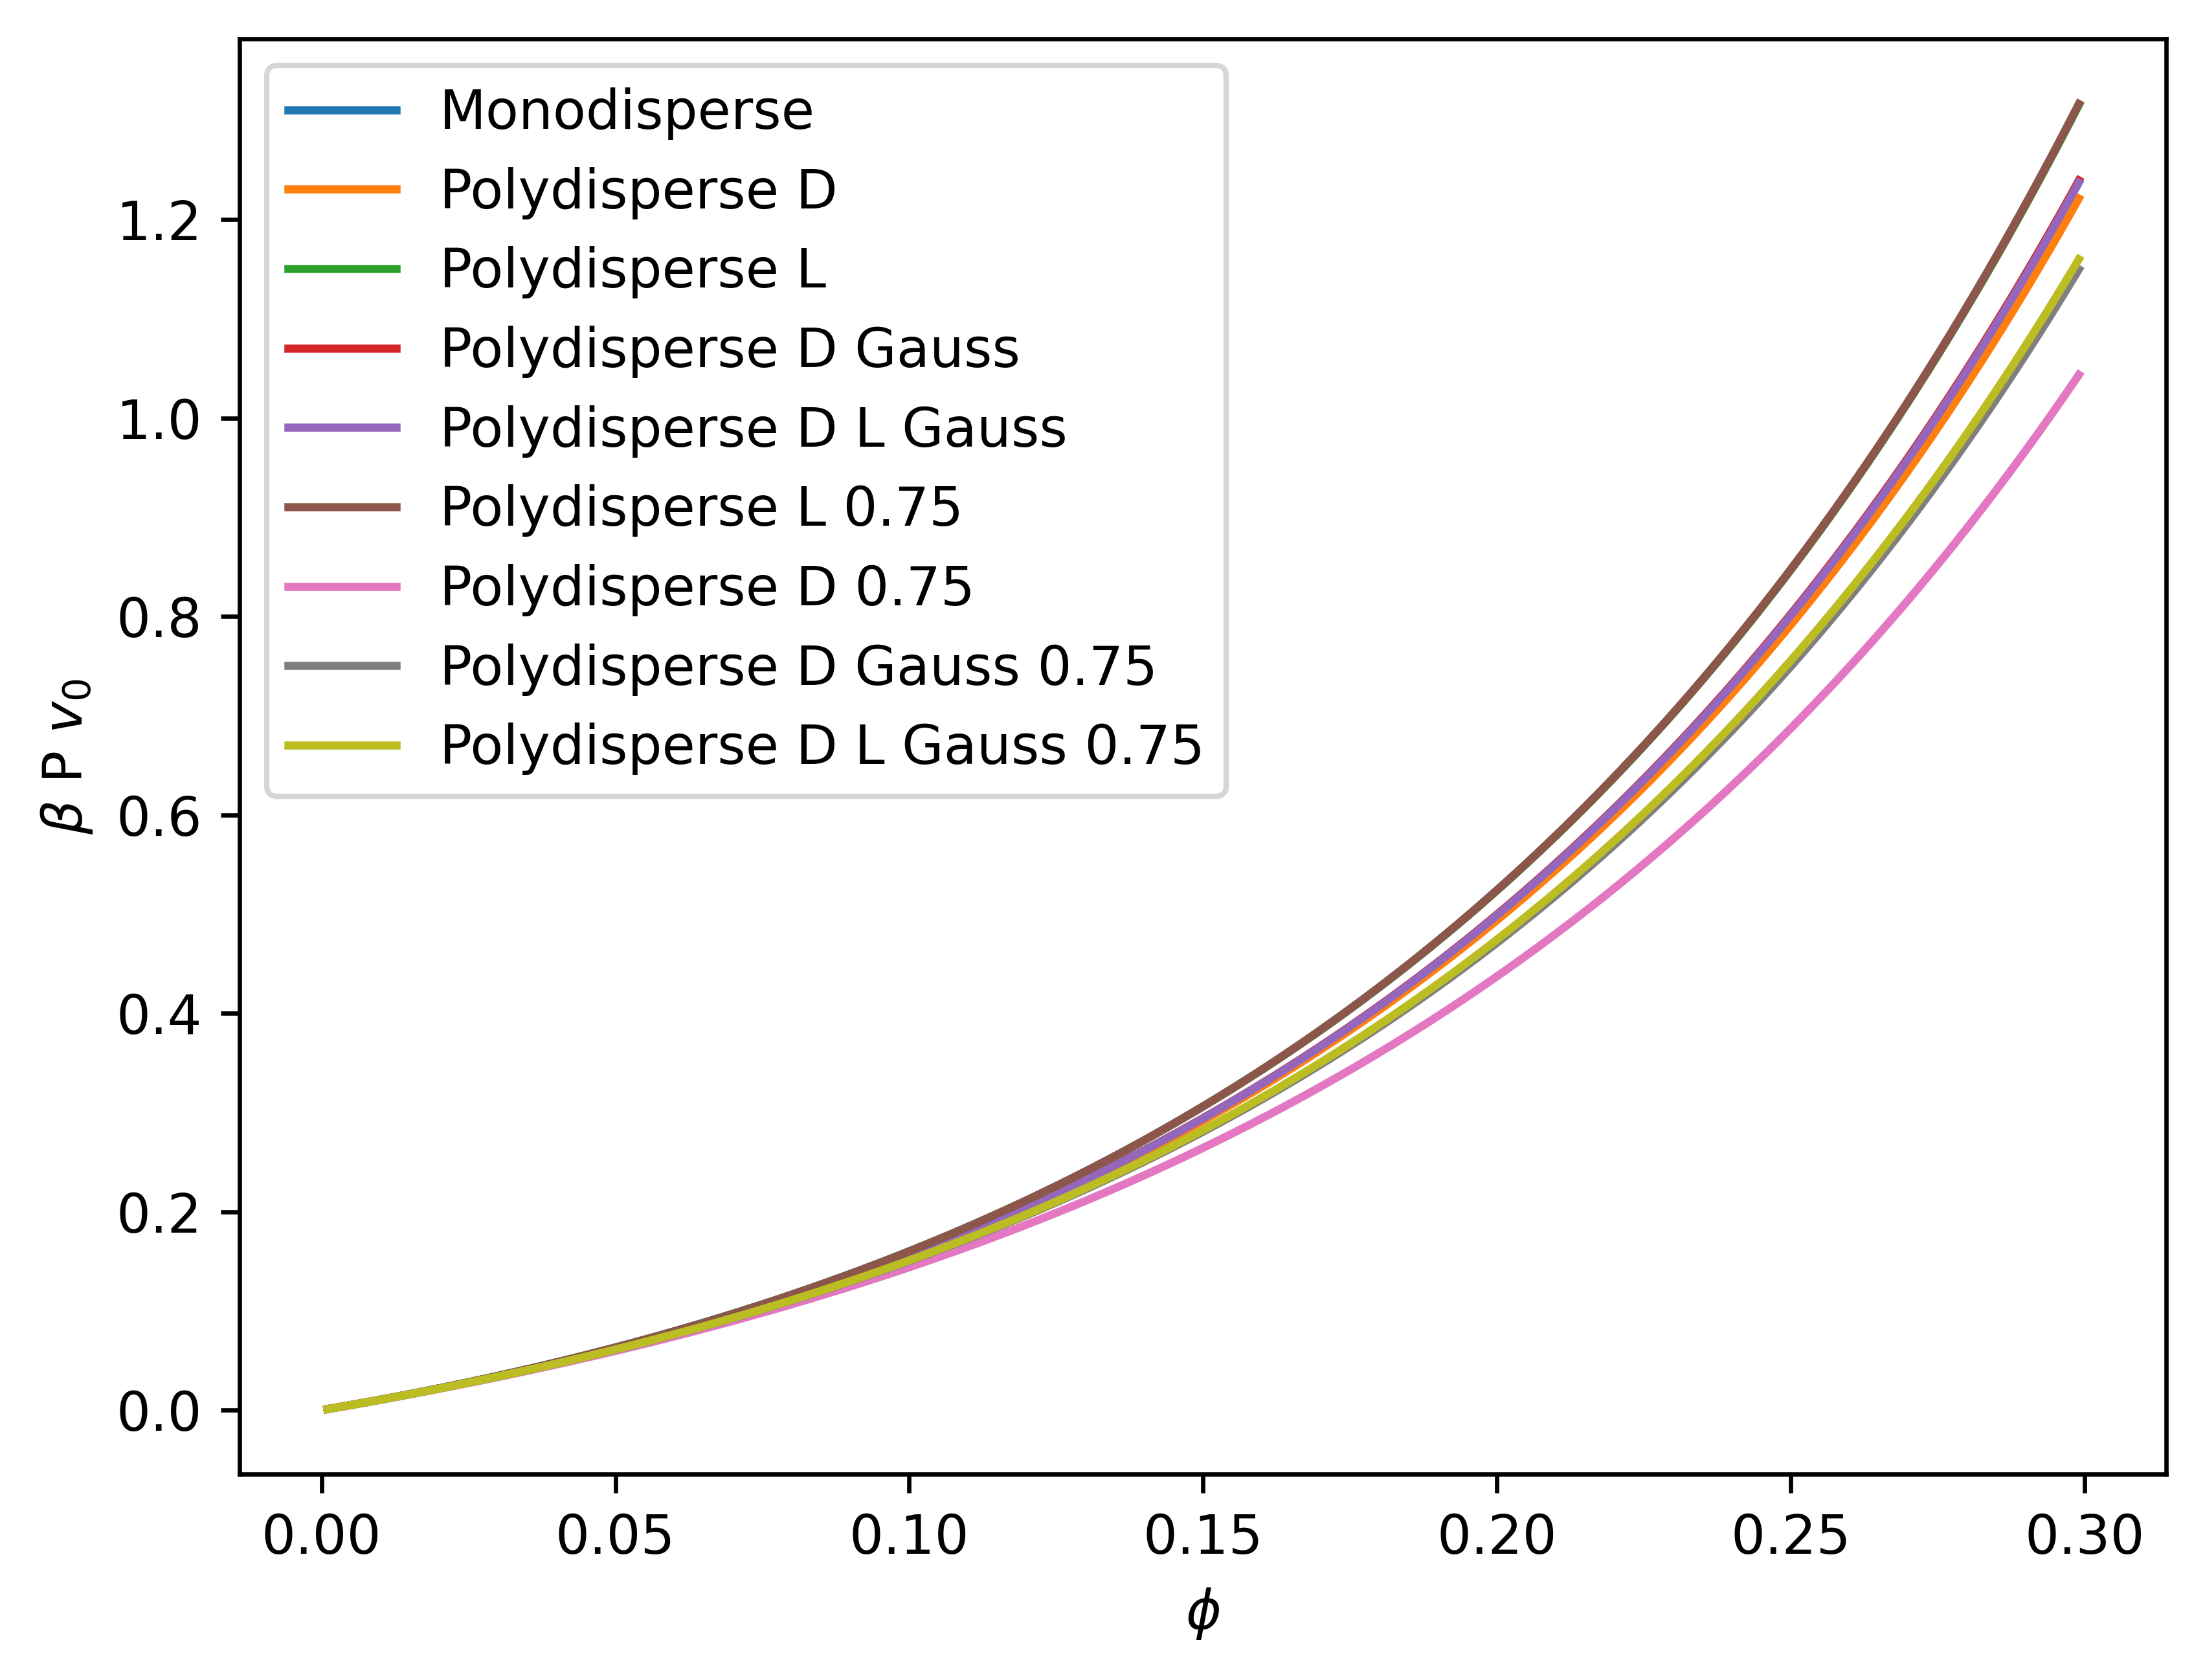
\includegraphics[width=0.45 \columnwidth]{Figures/EOS_TH_A1.png}
	\includegraphics[width=0.45 \columnwidth]{Figures/EOS_TH_A5.png}
	\caption{Theoretical EOS of the systems in the case of $\overline{A} = 1$ (left) and $\overline{A} = 5$ (right).}
	\label{fig:TH_EOS}
\end{figure}

Strikingly, while the numerical comparison between EOS obtained through simulations and theoretically is only qualitative, the deviation between the monodisperse and polydisperse predicted packing fractions for all of the analysed cases is quantitative, as can be see in figure \ref{fig:DeltaP_P}. 

\begin{figure}[!h]
	\centering
	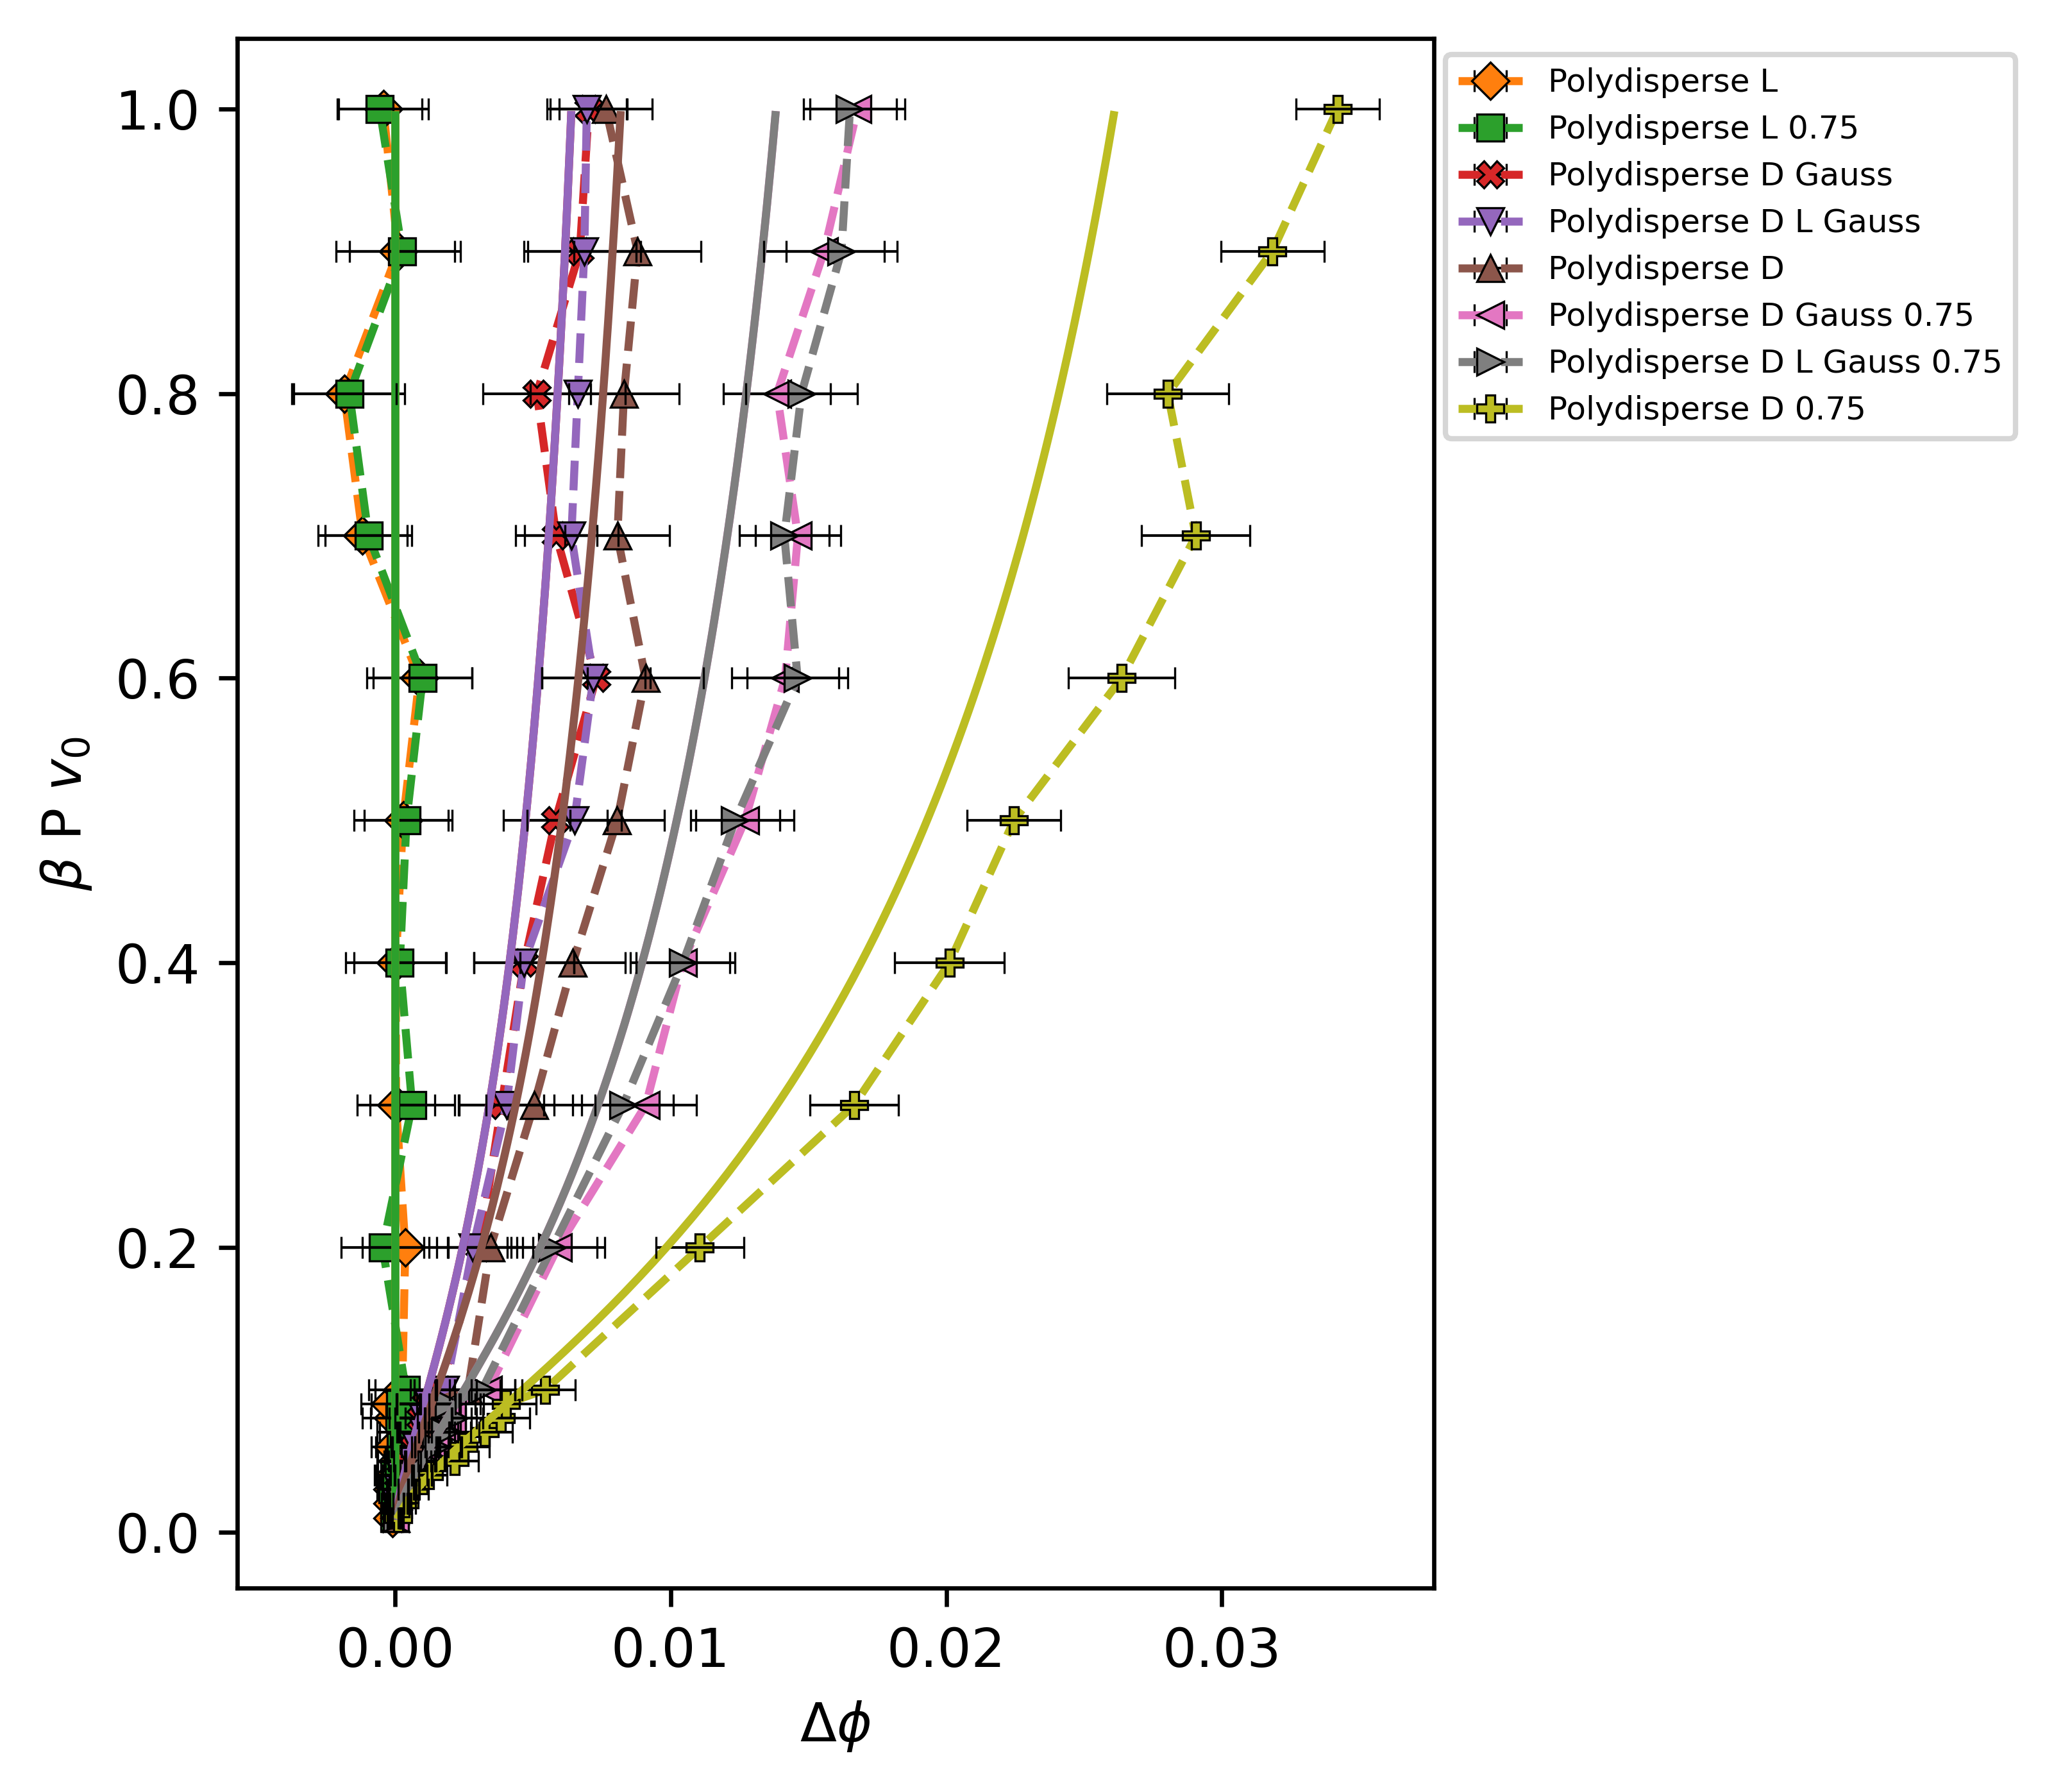
\includegraphics[width=0.45 \columnwidth]{Figures/Deltaphi_P_A1.png}
	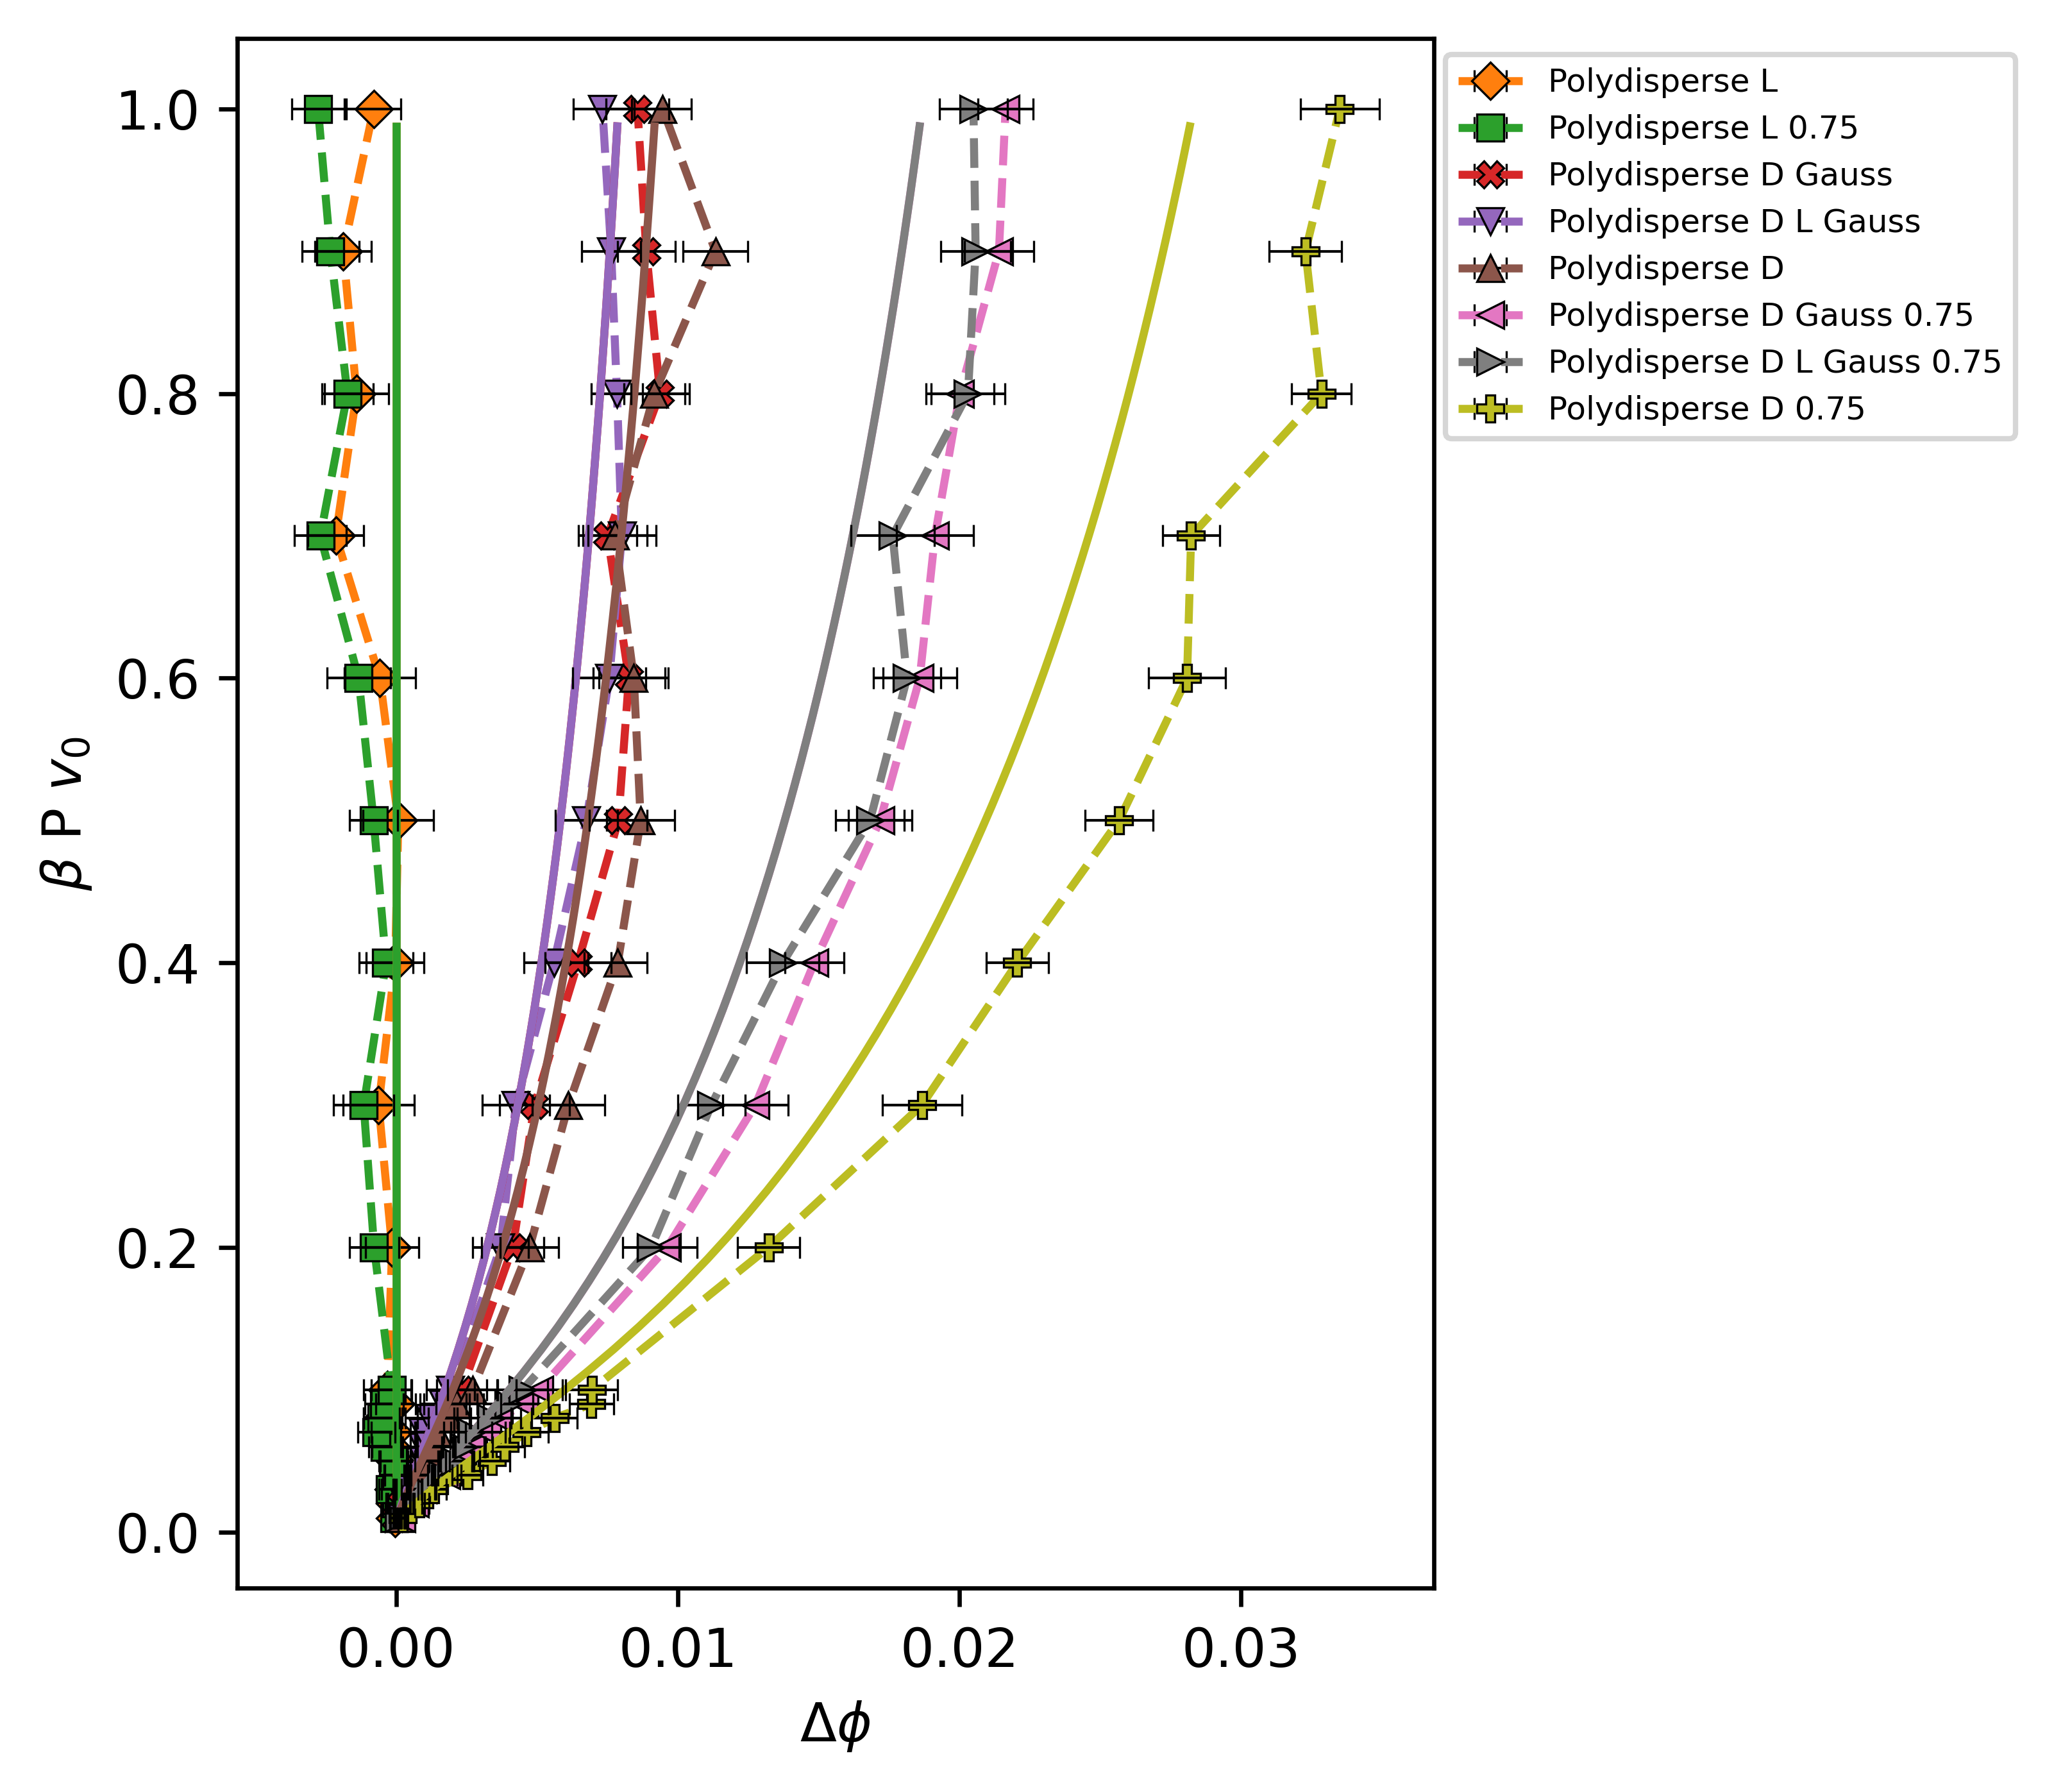
\includegraphics[width=0.45 \columnwidth]{Figures/Deltaphi_P_A5.png}
	\caption{Quantitative theory agreement. Difference between the polydisperse cases and the monodisperse one for the different systems analysed in this work for $\overline{A} = 1$ (left) and $\overline{A} = 5$ (right).}
	\label{fig:DeltaP_P}
\end{figure}

This result is on the one hand exciting as it implies that a simple theoretical calculation is able to predict qualitatively and quantitatively EOS in any  polydisperse system if the corresponding monodisperse one is known. 


%Secondly, we can analyse in depth the various contributions to $F$ to assess the reason underlying the independency of the EOS on a polydispersity in $L$, and evict why $D$ plays such a crucial role. As a matter of fact, the main term affecting the theoretical free energy is the ratio between the average excluded volume between all particles in solution, and mean particle volume $v_0$.


%\subsection{Theoretical I-N transition}



\section{Conclusions}


We then undergo an in depth analysis separating the $L$ and $D$ contributions to the polydisperse $A$ distribution. 
Interestingly, the change in compressibility of the polydisperse solution with respect to their monodisperse counterparts, is dominated by the  $D$ polydispersity, while even a $100\%$ polydispersity in $L$ does not change the  equation of state obtained for the monodisperse case. To explain such a phenomenon, we studied both global and local properties of the solutions, introducing global and orientational pair distribution functions. Such analyses showed the emergence of a local alignment between the elongated nanoparticles, even in dilute systems. 
%%%
%Qui aggiungiamo il commento sul fatto che sia il volume escluso a dominare - CONTROLLIAMO BENE 
%%%
We show that the more the nanoparticles are elongated, the higher is the local cooperativity in alignment. Moreover the average number of particles that are involved in the local pre-nematic ordering is higher the more anisotropic the particles  are.
Nevertheless such an effect is present both in polydisperse as well as in monodisperse systems. 
To understand why polidispersities in $D$ and $L$ play such a different role on the EOS, we  generalise, to the polydisperse case,  a standard theoretical tool that estimates the equation of state of the solutions through a mean field approach. We use the Parson Lee approximation for estimating the excluded volume effect on the free energy of the system, and analyse the effect of a set of different probability  distributions for $L$ and for $D$ on the equilibrium properties of the solutions. 
Even the theoretical approach shows a strong effect of the compressibility correlated to a polydispersity in $D$, while none of the considered distributions for the polydispersity in $L$ affect the EOS.  We notice that the free volume term is dominated by a $D^3$ contribution, while the strongest contribution arising from $L$ scales as $L^2$. This result seem to indicate that while the presence of anysotropy induce a preferential alignement between particles even at low $\phi$, the strongest effect on compressibility is linked to the excluded volume term. 

%In this paper is analysed the effect of polydispersity onto the low packing fraction phase diagram of functionalisable hard colloidal particles of various anisotropy. 

The paper is structured as follows: in the fist part, we estimate the monodisperse low packing fraction phase diagram for hard spherocylinders with  $A=L/D \in [1,5]$. We then introduce polydispersity on both $L$ and $D$, fixing the average $A$ to be comparable with the monodisperse case. Polydispersity is introduced on $A$, $D$ and $L$, and all contributions to the total polydispersity of the nanoparticles are analysed both globally as well as separately. This analysis demonstrates the predominant role of the polydispersity on $D$ on the equilibrium properties of the solutions, while a polydispersity in $L$ does not seem to have any effect on the packing of the nanoparticles for a given equilibrium pressures. 
We then introduce and generalise the Parson Lee approximation for the equation of state of elongated nanoparticles, to the case in which nanoparticles are polydisperse (generalising the calculation of the excluded volume term in the Excess Pressure to the polydisperse case), and compare the results obtained to the simulation results. Even if Parson Lee approximation is known to well reproduce the phase diagram at intermediate packing fraction, we show that the theoretical predictions at low packing fraction  worsen with increasing $A$, in all considered cases. Nevertheless the theoretical predictions underestimate by only about $10\%$ the worse case scenario. 
At last, we analyse both global and local properties of the solutions by computing the pair distribution functions between all particles, the nematic parameter, and the local orientational pair distribution function. 
While no nematic order is shown by any of the analysed systems in the considered range of the packing fraction, it is possible to appreciate the emergence of a local alignment between the nanoparticles that is enhanced by a higher value of $A$: as soon as $\phi >\phi^*$, local rotational freedom is lost and nanoparticles start aligning one with respect to the other. The local alignement involves a number of particles that is an increasing function of $A$: the more the nanoparticles are anisotropic the higher the number of particles that start aligning locally one with respect to the other.   
From the analysis of the pair distribution function between all particles, it is shown that solutions of slightly anisotropic particles behave similarly to solution of spherical colloids, so that a fluid phase emerges, as $A$ increases, the homogemeous liquid like behaviour is lost.  
The emergence of local alignment between particles is part of the explanation on  why the polydisperse phase diagram for low $\phi$ is almost unaffected by a polydispersity in $L$ and dominated by the polydispersity in $D$: as particles align locally but, no global nematic order arises due to the low concentrations, the ``noise'' introduced by polydispersity on $L$ is not felt by the global properties of the solution, while the one on $D$ affects the average distance between the slightly oriented clusters of particles, thus affecting the global compressibility of the system. 
%%%
% questa va meglio
%%%
This is corroborated by the theoretical approach, that highlights how the excluded volume term - that is dominated bu $D$, affects the EOS



\begin{comment}
Polidispersita in D0.75 puo essere perche e' troppo asimmetrica la distribuzione in A e quindi il sistema e' al limite di una separazione di fase?  secondo me po esse




ISTRUZIONI IMMAGINI:
FAI FIGURE CON MENO TICS E CON FONT PIU GRANDI E SENZA LEGENDA NELLA FIGURA

FAI 
g(r) A=1 A=5
g2(r)  (taglia a 8)



PARSON LEE A=1 A=5 e paragone con simulazioni 

delta phi vs phi  per tutti simulazioni e teo tutte ma A=1, A=5 nel testo altre negli SI
\end{comment}












%%%%%%%%%%%%%%%%%%%%%%%%%%%%%%%%%%%%%%%%%%%%%%%%%%%%%%%%%%%%%%%%%%%%%
%% The "Acknowledgement" section can be given in all manuscript
%% classes.  This should be given within the "acknowledgement"
%% environment, which will make the correct section or running title.
%%%%%%%%%%%%%%%%%%%%%%%%%%%%%%%%%%%%%%%%%%%%%%%%%%%%%%%%%%%%%%%%%%%%%
\begin{acknowledgement}

The Grant of Excellence Departments, MIUR-Italy (ARTICOLO 1, COMMI 314 - 337 LEGGE 232/2016) is gratefully acknowledged.

\end{acknowledgement}


%%%%%%%%%%%%%%%%%%%%%%%%%%%%%%%%%%%%%%%%%%%%%%%%%%%%%%%%%%%%%%%%%%%%%
%% The same is true for Supporting Information, which should use the
%% suppinfo environment.
%%%%%%%%%%%%%%%%%%%%%%%%%%%%%%%%%%%%%%%%%%%%%%%%%%%%%%%%%%%%%%%%%%%%%

\begin{comment}
\begin{suppinfo}

This will usually read something like: ``Experimental procedures and
characterization data for all new compounds. The class will
automatically add a sentence pointing to the information on-line:

\end{suppinfo}
\end{comment}

\bibliography{polyhsc}


%%%%%%%%%%%%%%%%%%%%%%%%%%%%%%%%%%%%%%%%%%%%%%%%%%%%%%%%%%%%%%%%%%%%%
%% The appropriate \bibliography command should be placed here.
%% Notice that the class file automatically sets \bibliographystyle
%% and also names the section correctly.
%%%%%%%%%%%%%%%%%%%%%%%%%%%%%%%%%%%%%%%%%%%%%%%%%%%%%%%%%%%%%%%%%%%%%
%\bibliography{achemso-demo}

\end{document}


